% ==================================================================
% MEMORIA DEL TFM — Sistema IoT Edge para mantenimiento predictivo
% Máster Universitario en Internet das Cousas (MUIoT) — UDC
% Autor: Sergio Villodas Zapata · Tutor: Tiago Manuel Fernández Caramés
%
% Compilar:  latexmk -pdf memoria_TFM.tex   (desde este directorio)
% NO MODIFICAR: tfm-muiot.sty, IEEEtran.bst, logo_*.pdf (plantilla oficial)
% El contenido vive en capitulos/ — este fichero solo lo ensambla.
% ==================================================================
\documentclass[%
    paper=A4,               % Tamaño de papel A4
    twoside,                % Páginas pares e impares con diseño diferenciado
    parskip=full,           % Renglón libre entre párrafos
    12pt,                   % Tamaño de fuente. No inferior a 12 puntos
    titlepage=on,           % Página independiente para el título
    captions=tableabove,    % Los títulos de las tablas en la parte superior
]{book}

% **************************************************
% * Idioma: galician, spanish, english
% **************************************************
\usepackage[spanish]{babel}

% **************************************************
% * Universidad: uvigo, udc, usc
% **************************************************
\usepackage[udc]{tfm-muiot}

% **************************************************
% * Diagramas. Añadido para el diagrama de bloques de la arquitectura
% * (capitulos/05-diseno.tex). No forma parte de la plantilla oficial.
% **************************************************
\usepackage{tikz}
\usetikzlibrary{arrows.meta, positioning, fit, backgrounds}

% **************************************************
% * Datos para la portada
% **************************************************
\title{Sistema IoT Edge para mantenimiento predictivo de compresores de refrigeración}
\author{Sergio Villodas Zapata}
\advisor{Tiago Manuel Fernández Caramés}
\course{2025/2026}

% **************************************************
% * Cabeceras (opcionales). Se activan con "true"
% **************************************************
\headers{true}

% **************************************************
% * Inicio del documento
% **************************************************
\begin{document}

\maketitle
\clearemptydoublepage

% **************************************************
% * Dedicatoria
% **************************************************
\dedication{Dedicatoria}
\clearemptydoublepage

% **************************************************
% * Tabla de contenidos
% **************************************************
\tableofcontents
\clearemptydoublepage

% **************************************************
% * Contenido — estructura obligatoria (Guía, apdo. 3)
% * Extensión objetivo: 25-50 páginas sin contar anexos
% **************************************************
% A. Introducción al problema (Guía apdo. 3.A)
% Extensión orientativa: 3-4 páginas
\chapter{Introducción}
\label{cap:introduccion}

La monitorización de activos críticos resulta fundamental para garantizar la operatividad
y prevenir averías inesperadas en entornos que abarcan desde el sector servicios hasta el
industrial. Los sistemas electromecánicos de refrigeración constituyen un caso
representativo: operan de forma continua, su fallo implica la pérdida del producto
conservado y su degradación rara vez es instantánea, sino que viene precedida por cambios
progresivos en su comportamiento físico.

% TODO: cuantificar el problema con fuentes citables (coste de la parada no planificada,
% porcentaje de fallos en compresores, ahorro atribuido al mantenimiento predictivo).
% Añadir las entradas correspondientes a referencias.bib en formato IEEE.

\section{Motivación}

El mantenimiento correctivo actúa una vez que el fallo ya se ha producido, mientras que el
mantenimiento preventivo basado en calendario sustituye componentes que a menudo conservan
vida útil. El mantenimiento predictivo se apoya en la medida continua de variables físicas
para estimar el estado real del activo y anticipar la intervención únicamente cuando el
comportamiento se desvía del nominal.

La adopción de este paradigma se ve limitada, en la práctica, por el coste de la
infraestructura de captura y por el volumen de datos que genera un muestreo de señales
mecánicas y acústicas. Enviar de forma continua señales de vibración a la nube resulta
costoso en ancho de banda y en almacenamiento, e introduce una dependencia de conectividad
que un activo industrial no siempre puede asumir.

\section{Planteamiento del problema}

Este trabajo aborda el diseño e implementación de un sistema de monitorización modular que
desplaza la lógica de diagnóstico hacia el extremo de la red (\textit{edge}). El nodo de
medida captura variables físicas del activo --vibración, temperatura y firma acústica-- y
el objetivo último es que la detección de anomalías se resuelva en el propio nodo, sin
depender de un flujo masivo de datos hacia la nube.

El activo seleccionado como escenario de prueba es el compresor de un sistema de
refrigeración, por su disponibilidad, su funcionamiento cíclico bien definido y la
posibilidad de inducir fallos controlados sin riesgo.

\section{Estructura del documento}

El capítulo~\ref{cap:estado-arte} analiza las necesidades del problema y el estado del arte
en mantenimiento predictivo e inteligencia en el borde. El capítulo~\ref{cap:objetivos}
detalla los objetivos perseguidos. El capítulo~\ref{cap:metodologia} describe la
metodología seguida de forma sucesiva. El capítulo~\ref{cap:diseno} justifica las
decisiones técnicas adoptadas, incluidos los estándares empleados. El
capítulo~\ref{cap:resultados} presenta los resultados obtenidos y el
capítulo~\ref{cap:conclusiones} recoge la discusión, las conclusiones y las líneas futuras.
Los anexos técnicos completan la información de detalle del sistema construido.
      % A. Introducción al problema
% B. Análisis de necesidades y estudio del estado del arte (Guía apdo. 3.B)
% Extensión orientativa: 5-7 páginas. Capítulo con mayor densidad de citas IEEE.
\chapter{Análisis de necesidades y estado del arte}
\label{cap:estado-arte}

\section{Análisis de necesidades}

El sistema debe satisfacer los siguientes requisitos, derivados del escenario de aplicación:

\begin{itemize}
    \item \textbf{Captura multivariable.} Un único tipo de señal no basta para discriminar
        modos de fallo: la vibración revela desequilibrios mecánicos, la temperatura revela
        pérdidas de rendimiento térmico y la firma acústica revela anomalías del régimen de
        giro.
    \item \textbf{Resiliencia mecánica.} El nodo opera acoplado a un elemento en vibración
        permanente, lo que degrada conexiones y cableado. El sistema debe seguir midiendo
        ante fallos físicos transitorios.
    \item \textbf{Operación autónoma prolongada.} La construcción del modelo de
        comportamiento nominal exige campañas de captura de días, sin supervisión.
    \item \textbf{Independencia de la nube.} El diagnóstico debe poder resolverse en el
        nodo, con la infraestructura externa limitada al entrenamiento y al análisis.
    \item \textbf{Coste contenido.} La solución debe construirse con componentes de bajo
        coste para resultar aplicable a activos de valor moderado.
\end{itemize}

\section{Mantenimiento predictivo basado en señales físicas}

La monitorización de condición de máquina rotativa se apoya en un conjunto de indicadores
consolidado, cuya elección responde a que cada uno resulta sensible a una familia distinta de
mecanismos de fallo~\cite{randall2011}. Esa correspondencia entre indicador y mecanismo es la
que justifica la selección de características descrita en el capítulo~\ref{cap:diseno}.

El valor eficaz de la componente alterna de la aceleración constituye el indicador de
severidad global. Su evolución es monótona con la degradación, lo que lo hace adecuado para
seguimiento de tendencia, y existen criterios normativos que relacionan su magnitud con
estados admisibles de la máquina según su clase~\cite{iso20816}. Su limitación es la
contrapartida de esa robustez: al promediar sobre toda la ventana, atenúa los eventos poco
frecuentes.

La kurtosis cubre precisamente ese hueco. Al ser el cuarto momento normalizado de la
distribución de amplitudes, cuantifica la impulsividad de la señal y no su magnitud, con lo
que responde a la aparición de impactos aislados antes de que estos alteren el valor
eficaz~\cite{randall2011}. Es el indicador clásico del deterioro incipiente de rodamientos, y
su interpretación se apoya en dos valores de referencia analíticos: 3 para ruido gaussiano y
1,5 para una señal senoidal pura. El par formado por el valor eficaz y la kurtosis discrimina
así entre mecanismos que un único indicador confundiría: un desequilibrio de masa eleva el
primero manteniendo el segundo próximo al de una senoide, mientras que un rodamiento en
deterioro incipiente apenas altera el primero y sin embargo eleva el segundo.

El análisis espectral aporta la dimensión que los indicadores temporales no pueden ofrecer: la
localización en frecuencia. La componente correspondiente a la frecuencia de giro y la
relación entre esta y sus armónicos permiten distinguir desequilibrio de masa, desalineación
y aflojamiento del anclaje, mecanismos que producen niveles globales semejantes pero
distribuciones espectrales distintas~\cite{randall2011}.

Procede señalar una condición que la literatura recoge y que resultó determinante en este
trabajo: la banda de frecuencias efectivamente utilizable no la fija el sensor sino su
montaje. La fijación del acelerómetro sobre la superficie a medir constituye un sistema
elástico cuya resonancia limita el intervalo en que la medida es fiel, y existen criterios
normalizados para el montaje precisamente por esa razón~\cite{iso5348}. El
capítulo~\ref{cap:resultados} documenta la magnitud de ese efecto en el montaje empleado.

La monitorización acústica se plantea como modalidad complementaria y no como alternativa. Su
interés reside en que un micrófono capta la señal radiada al aire sin requerir contacto
mecánico, lo que la hace sensible a fenómenos que la vibración estructural no transmite bien,
como la obstrucción del caudal de aire. Su inconveniente, contrastado experimentalmente en
este trabajo, es que un micrófono solidario a la estructura recibe la vibración por conducción
y deja de medir el aire.

\section{Inteligencia en el borde de la red}

La ejecución de modelos de aprendizaje automático sobre microcontroladores de bajo consumo
constituye un campo con denominación propia, habitualmente designado como \textit{TinyML}, y
su desarrollo responde a restricciones que no aparecen en los entornos de cómputo
convencionales: memoria del orden de decenas o centenares de kilobytes, ausencia de sistema
operativo de propósito general y presupuesto energético acotado~\cite{warden2019}. Las
herramientas que han hecho practicable ese despliegue, en particular los entornos de
ejecución de modelos reducidos para microcontroladores, prescinden de asignación dinámica de
memoria y de gran parte del repertorio de operadores de sus equivalentes de
servidor~\cite{david2021}.

Conviene precisar el alcance de esas herramientas, porque condiciona la solución que se adopta
en el capítulo~\ref{cap:resultados}. Su repertorio de operadores corresponde a
\textbf{redes neuronales}: convoluciones, capas densas y funciones de activación. Un modelo que
no pertenezca a esa familia —una envolvente estadística, un método basado en vecindad, un
conjunto de árboles— no es ejecutable en ellas, de modo que su despliegue sobre el
microcontrolador exige programarlo directamente. La disponibilidad de un entorno de inferencia
no es por tanto un requisito del cómputo en el borde, sino una facilidad aplicable a una
familia concreta de modelos.

El contraste con una arquitectura orientada a la nube resulta cuantificable en el caso que
nos ocupa, y no es una cuestión de preferencia. Transmitir la señal de vibración en bruto de
los tres ejes a la frecuencia que exige el análisis frecuencial supone del orden de 3000
valores por segundo de forma continua. Extraer las características en el nodo y transmitir
únicamente estas reduce el volumen a un mensaje cada \mbox{30 s}, tres órdenes de magnitud por
debajo. La diferencia no afecta solo al ancho de banda: condiciona la autonomía del nodo, el
coste de almacenamiento y, sobre todo, la dependencia operativa de un enlace externo.

Esa última consideración es la que motiva el planteamiento de este trabajo. Un sistema de
diagnóstico cuya lógica reside en un servidor remoto deja de diagnosticar cuando el enlace
falla, circunstancia que en un entorno industrial no es excepcional. Situar la inferencia en
el nodo convierte la infraestructura externa en soporte de entrenamiento y análisis en lugar
de requisito de operación.

Conviene precisar que el planteamiento no exige necesariamente una red neuronal. Cuando el
problema admite una formulación estadística, el modelo embarcado puede reducirse a un
conjunto de parámetros de unos pocos kilobytes, sin la infraestructura de un entorno de
ejecución de aprendizaje automático. El capítulo~\ref{cap:diseno} desarrolla esta alternativa
y su justificación.

\section{Detección de anomalías no supervisada}

La formulación del problema de detección responde a una asimetría en la disponibilidad de
datos que es característica del mantenimiento predictivo. De un activo en servicio se obtiene
con facilidad un registro extenso de su comportamiento normal, mientras que los ejemplos de
fallo son escasos, difíciles de etiquetar y, cuando se obtienen de forma deliberada, costosos.
Un clasificador supervisado requeriría un número de ejemplos de cada modo de fallo que no es
alcanzable en este contexto, de modo que el planteamiento adecuado es el de detección de
anomalías con una sola clase: el modelo se ajusta exclusivamente sobre el estado nominal y
señala como anómala toda observación suficientemente alejada de la región que ha aprendido a
describir.

Entre los métodos aplicables destaca por su idoneidad el basado en árboles de aislamiento, que
en lugar de modelar la densidad de la distribución normal explota que las observaciones
anómalas resultan más fáciles de separar del resto mediante particiones
aleatorias~\cite{liu2008}. Su interés práctico reside en un coste computacional reducido y en
que no requiere estimar una densidad en un espacio de características de dimensión elevada,
condición que otros métodos encuentran problemática.

La alternativa clásica formula el problema como la estimación del soporte de una distribución
de dimensión elevada, buscando la frontera que encierra la fracción especificada de los datos
de entrenamiento~\cite{scholkopf2001}. Su comportamiento depende de la elección del núcleo y
de sus parámetros, y su coste crece con el número de observaciones, lo que la hace menos
conveniente cuando el conjunto de referencia es extenso.

Procede añadir dos métodos que el desarrollo de este trabajo mostró pertinentes y que la
formulación inicial no contemplaba. El primero estima la densidad local de cada observación y la
compara con la de su vecindad, con lo que declara atípico aquello que reside en una región
menos poblada que su entorno inmediato~\cite{breunig2000}. Su interés en este caso reside en
que no presupone una forma concreta para la distribución del estado nominal, circunstancia
favorable cuando ese estado agrupa condiciones de operación heterogéneas, como son los ciclos
de marcha de duración desigual de un compresor sometido a uso doméstico.

El segundo ajusta una envolvente elipsoidal mediante una estimación robusta de la matriz de
covarianza, obtenida a partir del subconjunto de observaciones de menor determinante, lo que
impide que unas pocas observaciones atípicas del propio conjunto de ajuste desplacen la
frontera~\cite{rousseeuw1999}. Su ventaja para el objetivo de este trabajo es que la regla de
decisión resultante es una forma cuadrática con parámetros precalculados, ejecutable en el nodo
con una ocupación de memoria del orden de centenares de bytes.

Una tercera vía la constituyen los autocodificadores, que se entrenan para reconstruir la
señal de entrada y emplean el error de reconstrucción como puntuación de anomalía. Su ventaja
es que encajan de forma natural en los entornos de ejecución para microcontroladores, dado
que son redes neuronales; su inconveniente, un coste de entrenamiento y una necesidad de datos
superiores a los de los dos métodos anteriores.

En los tres casos, la decisión final descansa sobre un umbral aplicado a una puntuación
escalar. Fijar ese umbral sobre un percentil de la distribución de puntuaciones del propio
conjunto nominal hace explícita y ajustable la tasa de falsos positivos admitida, lo que
resulta preferible a un valor arbitrario.

\section{Síntesis y aportación de este trabajo}

Los trabajos revisados abordan por separado las tres cuestiones que este proyecto integra: los
indicadores de condición sobre señal de vibración, el despliegue de inferencia en
microcontroladores y la detección de anomalías con una sola clase. La combinación de las tres
sobre una plataforma de coste reducido está menos explorada, y es donde este trabajo pretende
aportar.

Existe además una circunstancia que la literatura consultada tiende a no abordar, y que en la
práctica de este proyecto resultó ser la determinante. Los métodos de monitorización de
condición se formulan asumiendo instrumentación de calidad y adquisición fiable: acelerómetros
acoplados de forma rígida y una cadena de medida que entrega las muestras que se le piden. Al
trasladar esos métodos a hardware de prototipado adherido a una máquina en vibración, ninguna
de las dos premisas se cumple. El bus de comunicación con el sensor falla de forma
intermitente, la fijación del acelerómetro introduce una resonancia que limita la banda
utilizable, y ambos efectos degradan precisamente los indicadores más sensibles.

La aportación de este trabajo se sitúa por tanto en dos planos. En el primero, la integración
de tres modalidades de sensado de bajo coste con extracción de características e inferencia en
el propio nodo. En el segundo, y con mayor valor práctico, la documentación cuantificada de
las limitaciones que impone ese hardware y de los mecanismos que permiten operar con ellas: la
validación de la integridad del dato en la adquisición, la instrumentación que hace medible la
calidad de cada medida, y la acotación explícita de la banda de frecuencias en que las
características resultan interpretables. El capítulo~\ref{cap:conclusiones} valora en qué
medida esas limitaciones condicionan el alcance alcanzado.
   % B. Análisis de necesidades y estado del arte
% C. Objetivos (Guía apdo. 3.C)
% Extensión orientativa: 2-3 páginas
\chapter{Objetivos}
\label{cap:objetivos}

\section{Objetivo general}

Diseñar e implementar un sistema modular de monitorización que emplee técnicas de
aprendizaje automático para el diagnóstico preventivo de sistemas electromecánicos,
analizando variables físicas --vibración, temperatura y sonido-- con el fin de identificar
desviaciones respecto al funcionamiento nominal del activo, y desplazando la lógica de
diagnóstico al extremo de la red.

\section{Objetivos específicos}

Los objetivos específicos se corresponden con las tareas comprometidas en la solicitud de
asignación de tema del presente TFM:

\begin{enumerate}
    \item \textbf{Definición del escenario de prueba.} Identificar un activo
        representativo y caracterizar su firma operativa.
    \item \textbf{Diseño de la arquitectura del sistema.} Definir el modelo de intercambio
        de datos entre los nodos sensores y la plataforma de monitorización, priorizando la
        eficiencia en el procesamiento local.
    \item \textbf{Selección de componentes de hardware y software.} Elegir la plataforma de
        procesado y los sensores adecuados para la captura de señales con la precisión
        requerida.
    \item \textbf{Desarrollo del motor de análisis inteligente.} Implementar algoritmos de
        aprendizaje automático para la extracción de características y la clasificación
        automática de los estados de salud del sistema monitorizado.
    \item \textbf{Validación experimental.} Realizar pruebas en un entorno controlado para
        calibrar el sistema y verificar la precisión del diagnóstico ante distintos tipos
        de fallo.
    \item \textbf{Pruebas en entorno real.} Desplegar una prueba de concepto sobre un
        activo operativo para validar la robustez de la arquitectura en condiciones de uso
        diario.
\end{enumerate}

\section{Alcance y limitaciones}

El trabajo se limita a dos activos de prueba: un compresor de referencia en estado nominal, sobre
el que se ajusta el modelo y se despliega el nodo, y un segundo compresor con una avería
preexistente que constituye el conjunto de evaluación. De ello se sigue la limitación de mayor
peso, desarrollada en el capítulo~\ref{cap:resultados}: al proceder la evidencia de detección de
una \textbf{máquina distinta} de aquella con la que se entrenó, el contraste no separa el efecto
del fallo del de la variabilidad entre ejemplares. Sobre el activo de referencia solo se
indujeron perturbaciones \textbf{operativas y ambientales} —reversibles y sin daño para la
máquina—, no fallos mecánicos. No se persigue tampoco la certificación metrológica de las
medidas: los sensores empleados son de bajo coste y las magnitudes se utilizan como indicadores
relativos de desviación, no como valores absolutos calibrados.

Procede acotar el alcance del motor de análisis en los términos en que efectivamente se ha
desarrollado. La propuesta de trabajo enuncia la clasificación automática de los estados de
salud; lo abordado es la \textbf{detección de una clase}, es decir el ajuste de un modelo del
estado nominal y la señalización de cuanto se desvíe de él, sin atribución de la desviación a un
estado concreto. La decisión responde a que un clasificador requiere ejemplos etiquetados de
cada estado, y los modos de fallo de un activo de esta naturaleza son escasos, variados y no
conocidos de antemano. La justificación detallada figura en el capítulo~\ref{cap:resultados}.

Tampoco se persigue el empleo de un entorno de ejecución de modelos reducidos para
microcontroladores. Esos entornos operan sobre redes neuronales, y el tamaño de muestra
alcanzable en una campaña de esta duración no permite ajustar una arquitectura de ese tipo sin
sobreajuste. La inferencia en el nodo se programa por tanto de forma directa, lo que no supone
una limitación del alcance sino una consecuencia de la familia de modelos aplicable.
         % C. Objetivos
% D. Metodología desarrollada de forma sucesiva (Guía apdo. 3.D)
% Extensión orientativa: 4-5 páginas. Narrar las fases EN ORDEN, incluidos los problemas
% encontrados y cómo se resolvieron: es lo que evidencia el trabajo realizado.
% Fuente de verdad del avance: docs/ROADMAP.md
\chapter{Metodología}
\label{cap:metodologia}

El desarrollo se organizó en fases sucesivas, cada una condicionada por el resultado de la
anterior. Este capítulo describe esa progresión, incluidas las incidencias encontradas y
las soluciones adoptadas.

\section{Fase 1: definición del escenario y de la arquitectura}

Se seleccionó como activo de prueba el compresor de un sistema de refrigeración doméstico y
se definieron las tres modalidades de sensado a integrar. Sobre esa base se estableció una
arquitectura de dos niveles: un nodo de captura en el borde y un concentrador local que
recibe la telemetría y construye el conjunto de datos.

\section{Fase 2: integración del nodo de sensado}

La integración se abordó de forma incremental, incorporando y validando un sensor cada vez
antes de combinarlos en un único ciclo de adquisición. El orden seguido fue: acelerómetro y
giroscopio sobre bus \textit{Inter-Integrated Circuit} (I\textsuperscript{2}C), sonda de
temperatura sobre bus 1-Wire y micrófono digital sobre bus \textit{Inter-IC Sound} (I2S).

\section{Fase 3: estabilización frente a la vibración}

Durante las primeras pruebas con el compresor en funcionamiento se detectó un fallo
recurrente: el bus I\textsuperscript{2}C quedaba bloqueado y el bucle principal del
microcontrolador se detenía indefinidamente. El origen se localizó en microcortes del
cableado del acelerómetro provocados por la propia vibración del activo, precisamente la
magnitud que el sistema debe medir.

La solución adoptada fue una rutina de detección y recuperación por software: en cada ciclo
se comprueba el reconocimiento del dispositivo en su dirección de bus y, si no responde, se
reinicia el bus y se reinicializa el sensor sin reiniciar el microcontrolador. Se descartó
de forma deliberada la alternativa de reiniciar el nodo, dado que un reinicio interrumpe la
continuidad temporal de la señal, que es la información que el análisis posterior explota.

\section{Fase 4: conectividad y almacenamiento}

Al preparar la primera campaña de captura prolongada se identificó una limitación en el
esquema de adquisición que habría invalidado el análisis previsto. El bucle de medida
operaba a una cadencia de \mbox{1 Hz}, suficiente para las magnitudes térmicas pero dos
órdenes de magnitud por debajo de lo que exige la vibración del activo, cuya componente
fundamental se sitúa en torno a los \mbox{48 Hz}. La consecuencia no era una pérdida de
precisión, sino la imposibilidad de todo análisis frecuencial: la señal se replegaba sobre la
banda observable.

La corrección consistió en desacoplar las dos escalas temporales del problema mediante dos
canales de adquisición con cadencias independientes, según se detalla en el
capítulo~\ref{cap:diseno}. El formato completo de las tramas de ambos canales, los valores
centinela que emplean y los procedimientos de aprovisionamiento y verificación del
concentrador se recogen en el anexo~\ref{anexo:software}. El bucle principal se reformuló además para no depender de
esperas activas prolongadas, y la conversión de la sonda de temperatura pasó a solicitarse de
forma asíncrona, dado que sus aproximadamente \mbox{750 ms} de conversión detenían el resto
de la adquisición.

Procede señalar que la limitación se detectó antes de lanzar la campaña de captura y no
después. De haberse iniciado la adquisición con el esquema anterior, las horas de medida
registradas no habrían contenido información espectral aprovechable y la campaña habría
debido repetirse por completo.

La validación del esquema de ráfagas se realizó en dos etapas deliberadamente separadas.
Las rutinas de extracción de características se implementaron sin dependencias del entorno
de ejecución del microcontrolador, lo que permitió verificarlas en un computador frente a
señales sintéticas de propiedades conocidas analíticamente. Solo después se comprobó su
comportamiento en la placa. El motivo de este orden es práctico: depurar operaciones
matemáticas a través del puerto serie del microcontrolador resulta desproporcionadamente
lento frente a hacerlo en un entorno de compilación local.

La verificación sobre la placa confirmó los dos parámetros críticos del esquema. La duración
real de la captura se mantuvo en \mbox{1024 ms} sin desviación apreciable en todas las
ráfagas observadas, lo que acredita que la cadencia de muestreo se sostiene y que el eje de
frecuencias resultante es válido. El cálculo completo de las características de los tres
ejes y de la ventana acústica consumió entre \mbox{29 ms} y \mbox{30 ms}, margen holgado
frente al periodo de \mbox{30 s} entre ráfagas. Se comprobó igualmente que, con el activo en
marcha, la frecuencia dominante coincidía en los tres ejes en torno a \mbox{49 Hz}, valor
compatible con el régimen de un motor de inducción de dos polos alimentado a \mbox{50 Hz} una
vez descontado el deslizamiento. Ese pico desaparecía con el compresor detenido, lo que
permitió atribuirlo al giro del motor y no a un acoplamiento eléctrico de la red.

\section{Fase 5: despliegue del concentrador}

El concentrador se implantó sobre una Raspberry~Pi que aloja el intermediario de mensajería
y el registrador. Durante la puesta a punto se constató que el equipo que alojaba el
intermediario cambió de subred en cuatro ocasiones, circunstancia problemática porque la
dirección del intermediario es una constante de compilación del firmware y cada cambio
obligaba a reprogramar el nodo.

La solución adoptada consistió en configurar la interfaz inalámbrica del concentrador como
punto de acceso, de forma que el nodo se conecte directamente a él sin encaminador
intermedio. El gestor de red asigna en ese modo una dirección fija, con lo que la constante
del firmware deja de depender de infraestructura ajena. La decisión aporta además dos
ventajas: el conjunto resulta portátil, al no requerir más que alimentación eléctrica, y la
red queda aislada, lo que elimina el riesgo de que un tercero publique tramas en los temas de
telemetría y contamine el conjunto de datos. Se asume como contrapartida que el concentrador
pierde su acceso a Internet por la interfaz inalámbrica, dado que esta no puede operar
simultáneamente como cliente y como punto de acceso; la gestión se mantiene por cable.

El aprovisionamiento se automatizó separando las operaciones en fases, por una razón de
seguridad operativa: la activación del punto de acceso interrumpe la red por la que llega la
sesión de administración remota. Todas las comprobaciones se realizan antes de modificar la
configuración del sistema, la activación del punto de acceso constituye la última operación y
se lanza desacoplada de la sesión para que se complete aunque la conexión se pierda.

El equipo empleado como concentrador contaba ya con un intermediario configurado para otros
usos. Se adoptó como criterio la intervención mínima: el procedimiento examina la
configuración existente y, cuando esta ya satisface los requisitos, no la modifica; cuando la
configuración ajena restringe el servicio a la interfaz local, se limita a informar sin
alterar ficheros de terceros. Ante cualquier fallo, restaura el estado anterior antes de
abortar. El fundamento es que dejar un servicio inoperativo en un equipo compartido resulta
más perjudicial que no haber intervenido.

La cadena completa se verificó eslabón por eslabón siguiendo el recorrido del dato: punto de
acceso activo, nodo asociado a la red, intermediario aceptando conexiones, tramas de ambos
canales recibidas, registrador en ejecución y ficheros de datos incrementando su número de
filas. Esta última comprobación se realiza contrastando el recuento de filas en dos instantes
separados, y no verificando la mera existencia del fichero, porque un fichero presente que no
crece constituye el modo de fallo más fácil de pasar por alto. Se comprobó asimismo que el
conjunto se restablece por completo tras un corte de alimentación sin intervención manual.

Las fases experimentales y los resultados obtenidos a partir de las campañas de captura
se recogen y analizan en detalle en el capítulo~\ref{cap:resultados}.

El preprocesado comprende dos filtrados de naturaleza distinta. El primero descarta los
valores centinela descritos en el capítulo~\ref{cap:diseno}, cuya inclusión distorsionaría
cualquier estadístico: un único valor de \mbox{$-127$ \textdegree C} arrastra la media de
temperatura de una jornada completa.

El segundo es consecuencia directa de las limitaciones del montaje documentadas en el
anexo~\ref{anexo:hardware}. Dado que se asume una tasa de fallo de lectura apreciable en
lugar de intervenir sobre el cableado, el conjunto de datos contendrá ráfagas de calidad
desigual, y el protocolo debe discriminarlas en lugar de tratarlas por igual. Los contadores
de salud que el nodo publica hacen posible ese filtrado sobre criterios objetivos: la
duración real de la captura permite descartar las ráfagas cuya cadencia no se sostuvo, y el
número de reintentos de cada ráfaga califica su calidad individual. Se establece por tanto
como criterio metodológico que el filtrado del conjunto de datos se documente de forma
explícita, indicando qué fracción de las ráfagas se descartó y con qué umbral, dado que esa
fracción forma parte del resultado y no de su preparación.

Sobre las ráfagas retenidas se calculan las características derivadas que requieren
historia y que el nodo no puede obtener de una ventana aislada: el gradiente térmico, el
diferencial entre la temperatura de la superficie del compresor y la del ambiente, la
evolución de los armónicos respecto de la componente fundamental y la duración de los ciclos
de marcha y parada, deducida del canal lento.

El diferencial térmico merece una mención por su función en el diseño. Emplear la diferencia
entre la temperatura del activo y la del ambiente, en lugar de la temperatura absoluta,
elimina de la formulación la variación estacional: un compresor en estado nominal mantiene un
salto térmico semejante sobre el ambiente con independencia de la temperatura exterior. La
alternativa, un modelo que persiguiese esa deriva ajustándose de forma continua, resulta
inviable porque no puede distinguir una deriva ambiental lenta de una degradación igualmente
lenta. Se prefiere por ello eliminar la variable de confusión a compensarla.

La validación exige disponer de referencia de verdad, que en este contexto solo puede
obtenerse provocando los fallos de forma deliberada. Se establecieron cuatro modos, elegidos
por ser reversibles y por afectar a modalidades de medida distintas: desequilibrio de masa,
aflojamiento del anclaje, obstrucción de la ventilación y sobrecarga térmica. Los dos
primeros se manifiestan en la vibración, el tercero en las magnitudes térmica y acústica y el
cuarto en la evolución térmica y en el patrón de los ciclos de marcha.

El protocolo de cada campaña impone tres condiciones. La primera es que la campaña de
referencia en estado nominal precede a cualquier fallo inducido, por ser irreversible el
orden inverso. La segunda es que el montaje del sensor no se modifica entre campañas: dado
que la firma de vibración depende del punto y de la rigidez de la fijación, un remontaje
invalida la referencia y obliga a repetirla. La tercera es que toda campaña queda anotada con
su activo, condición, montaje, ficheros e incidencias, sin lo cual un fichero de datos carece
de las condiciones experimentales que le dan sentido.

La comparación se plantea dentro de un mismo activo, con estado nominal y estados de fallo
registrados sobre la misma máquina y el mismo montaje. Esta restricción excluye contrastar el
modelo ajustado sobre un activo frente a las medidas de otro distinto, procedimiento que no
permitiría discernir si una anomalía señalada corresponde al fallo o simplemente a la
diferencia entre máquinas.

El umbral de decisión se calibra sobre la distribución de puntuaciones del conjunto nominal,
lo que fija la tasa de falsos positivos admitida, y la evaluación se expresa mediante la
matriz de confusión frente a cada modo de fallo inducido.

La última fase traslada el sistema a un activo en uso diario, condición que introduce
perturbaciones ausentes en el banco: aperturas de puerta, variación de la carga térmica y
ciclos de desescarche. El objetivo no es mejorar la detección sino comprobar que el
comportamiento normal del activo, en toda su variabilidad, no genera una tasa de aviso
inaceptable.

Las métricas de robustez previstas son el tiempo de servicio sin intervención, la fracción de
ráfagas válidas sobre las esperadas, la evolución de los contadores de salud del nodo y la
tasa de avisos en ausencia de fallo conocido. Se incorpora además la comprobación de que el
veredicto de estado sigue siendo observable en el propio nodo con el concentrador apagado,
dado que la autonomía del extremo constituye la tesis del trabajo y afirmarla sin verificarla
carecería de fundamento.
       % D. Metodología desarrollada
% E. Decisiones técnicas, incluyendo normas y estándares o justificando su ausencia
% (Guía apdo. 3.E). Extensión orientativa: 6-8 páginas. Es el capítulo técnico central.
% Fuentes de verdad: docs/ARCHITECTURE.md, docs/DATA_SCHEMA.md, README.md (pinout)
\chapter{Diseño del sistema}
\label{cap:diseno}

\section{Arquitectura general}

El sistema se estructura en dos niveles. El nodo de borde, basado en un microcontrolador
ESP32, realiza la adquisición de las señales físicas y su empaquetado. El concentrador
local, implementado sobre un ordenador de placa reducida Raspberry~Pi, aloja el
intermediario de mensajería y el registrador que consolida el conjunto de datos destinado al
entrenamiento del modelo.

La figura~\ref{fig:arquitectura} recoge el flujo completo de la información. Conviene
subrayar la dirección de las flechas: el nodo transmite características ya calculadas y no
señal en bruto, y el concentrador devuelve al nodo un modelo entrenado. El sistema no es por
tanto una cadena lineal de sensor a servidor, sino un ciclo en el que el concentrador
interviene en la fase de entrenamiento y queda prescindible en la de explotación.

\begin{figure}[ht!]
\centering
\begin{tikzpicture}[
  font=\small,
  bloque/.style={draw, rounded corners=2pt, align=center, inner sep=6pt, minimum height=1cm},
  nodo/.style={bloque, fill=black!4, text width=4.4cm},
  hub/.style={bloque, fill=black!8, text width=4.4cm},
  activo/.style={bloque, fill=black!12, text width=2.6cm},
  flecha/.style={-{Latex[length=2mm]}, thick},
  etiq/.style={font=\scriptsize, align=center, inner sep=2pt}
]
  \node[activo] (activo) {Compresor\\(activo de prueba)};
  \node[nodo, right=2.4cm of activo] (nodo)
      {\textbf{Nodo de borde (ESP32)}\\[2pt]
       Adquisición multisensor\\
       Extracción de características\\
       Inferencia embarcada};
  \node[hub, right=2.4cm of nodo] (hub)
      {\textbf{Concentrador (Raspberry Pi)}\\[2pt]
       Intermediario MQTT\\
       Registrador a ficheros CSV\\
       Entrenamiento del modelo};

  \draw[flecha] (activo) -- node[etiq, above] {vibración\\temperatura\\sonido} (nodo);
  \draw[flecha] (nodo) -- node[etiq, above] {MQTT sobre\\Wi-Fi 2,4 GHz} (hub);
  \draw[flecha] (hub.south) -- ++(0,-0.9)
      node[etiq, below] {modelo entrenado (fase de despliegue)} -| (nodo.south);
  \draw[flecha] (nodo.north) -- ++(0,0.8)
      node[etiq, above] {veredicto de estado};
\end{tikzpicture}
\caption{Arquitectura del sistema. El nodo transmite características extraídas, no señal en
bruto; el concentrador entrena el modelo y lo devuelve al nodo, que ejecuta la inferencia.}
\label{fig:arquitectura}
\end{figure}

\section{Adquisición: sensores, plataforma y frecuencias de muestreo}

El cuadro~\ref{table:sensores} recoge los sensores seleccionados y la magnitud que aporta
cada uno al diagnóstico.

\begin{table}[ht!]
\caption{Sensores integrados en el nodo de borde.}
\label{table:sensores}
\centering
\begin{tabular}{|p{3cm}|p{2.6cm}|p{7cm}|}
\hline
\textbf{Sensor} & \textbf{Interfaz} & \textbf{Magnitud y aportación al diagnóstico} \\
\hline
MPU-6050~\cite{mpu6050} & I\textsuperscript{2}C & Aceleración en tres ejes y velocidad angular en tres
ejes; detecta desequilibrios mecánicos y aflojamiento del anclaje. Aporta además una
temperatura interna utilizada como indicador relativo. \\
\hline
DS18B20~\cite{ds18b20} & 1-Wire & Temperatura del entorno o de la tubería, con encapsulado metálico apto
para contacto; permite evaluar el rendimiento térmico del ciclo. \\
\hline
INMP441~\cite{inmp441} & I2S & Nivel acústico digital omnidireccional; la salida digital evita la
inmunidad reducida a la interferencia electromagnética propia de los micrófonos analógicos
en presencia de un motor. \\
\hline
\end{tabular}
\end{table}

La plataforma de procesado quedó condicionada por los buses que exigen esos sensores. Se
seleccionó el ESP32 por integrar en un mismo encapsulado los tres requeridos
(I\textsuperscript{2}C, 1-Wire por software e I2S nativo), conectividad inalámbrica y capacidad
de cómputo suficiente para ejecutar inferencia embarcada~\cite{esp32datasheet}, con un consumo y
un coste compatibles con el despliegue en activos de valor moderado. El
cuadro~\ref{table:requisitos} expresa esa elección en términos de requisitos medibles derivados
del propio sistema, en lugar de una preferencia general por la plataforma.

\begin{table}[ht!]
\caption{Requisitos de la plataforma de procesado, derivados del sistema implementado.}
\label{table:requisitos}
\centering
\begin{tabular}{|p{4.1cm}|p{2.4cm}|p{5.7cm}|}
\hline
\textbf{Requisito} & \textbf{Magnitud} & \textbf{Origen} \\
\hline
Entrada I2S nativa & --- & El micrófono es digital. Sin este periférico haría falta un
conversor externo, con la sensibilidad al ruido electromagnético que se pretendía evitar \\
\hline
Coma flotante en hardware & 5 transformadas de 1024 puntos en \mbox{30 ms} & Cada ráfaga
exige tres transformadas de vibración y dos de audio. La cifra corresponde a la medida en
la placa \\
\hline
Memoria de datos & \mbox{22,9 KiB} en reserva estática & Almacenes de ráfaga, de audio y de
trabajo de la transformada, dimensionados en tiempo de compilación \\
\hline
Conectividad inalámbrica integrada & \mbox{2,4 GHz} & Enlace con el concentrador. La banda
de \mbox{5 GHz} no es utilizable por el nodo \\
\hline
Capacidad de inferencia embarcada & --- & Requisito derivado del planteamiento del trabajo:
el diagnóstico debe poder ejecutarse sin el concentrador \\
\hline
\end{tabular}
\end{table}

Los dos primeros son los que efectivamente discriminan. La ausencia de entrada I2S nativa obliga
a incorporar un conversor analógico-digital externo, lo que reintroduce precisamente la
vulnerabilidad a la interferencia electromagnética que motivó la elección de un micrófono digital
en un entorno con un motor de inducción; la ausencia de unidad de coma flotante en hardware no
impide el cálculo pero obliga a reformular la transformada en aritmética de punto fijo, con el
consiguiente análisis de escalado y pérdida de precisión.

La reserva estática de \mbox{22,9 KiB} no es el consumo total del firmware sino solo el de los
almacenes de señal. Dimensionarlos en tiempo de compilación, en lugar de asignarlos de forma
dinámica, responde a que el nodo debe operar de forma continuada durante días: la asignación
dinámica repetida fragmenta el montón de memoria y termina provocando fallos que se manifiestan
tras horas de funcionamiento, cuando resultan más difíciles de diagnosticar.

Resuelta la plataforma, queda por fijar la cadencia de captura, que condiciona por completo el
análisis posterior y constituye la decisión técnica más restrictiva del sistema. El teorema del
muestreo establece
que para observar una componente de frecuencia $f$ es necesario muestrear por encima de
$2f$. Un compresor hermético accionado por un motor de inducción de dos polos alimentado a
\mbox{50 Hz} gira en torno a las \mbox{2900 RPM}, es decir, unas 48 vueltas por segundo, de
modo que su vibración presenta una componente fundamental próxima a los \mbox{48 Hz} junto
con sus armónicos.

Una cadencia de adquisición de \mbox{1 Hz}, adecuada para las magnitudes térmicas, sitúa el
límite de Nyquist en \mbox{0,5 Hz} y resulta por tanto dos órdenes de magnitud insuficiente
para la vibración. El efecto no es una medida degradada sino una medida carente de sentido
físico: la componente de \mbox{48 Hz} se repliega sobre la banda observable y aparece como
una frecuencia arbitraria sin relación con el régimen real del activo.

Transmitir de forma continua los tres ejes a la frecuencia requerida supondría del orden de
3000 valores por segundo, volumen incompatible con el enlace inalámbrico y contrario al
planteamiento del trabajo. La solución adoptada consiste en desacoplar las dos escalas
temporales del problema mediante dos canales de adquisición y publicación independientes,
según recoge el cuadro~\ref{table:muestreo}.

\begin{table}[ht!]
\caption{Canales de adquisición y sus parámetros de muestreo.}
\label{table:muestreo}
\centering
\begin{tabular}{|p{3.1cm}|p{2.2cm}|p{2.2cm}|p{4.6cm}|}
\hline
\textbf{Canal} & \textbf{Cadencia} & \textbf{Muestreo} & \textbf{Contenido} \\
\hline
\texttt{fridge/sensors} & \mbox{1 Hz} continuo & \mbox{1 Hz} & Nueve variables
instantáneas: temperaturas, aceleración, giro y nivel acústico \\
\hline
\texttt{fridge/vibration} & Una ráfaga cada \mbox{30 s} & \mbox{1 kHz} (vibración),
\mbox{16 kHz} (audio) & Características temporales y espectrales extraídas de 1024
muestras por eje \\
\hline
\end{tabular}
\end{table}

La ráfaga de 1024 muestras a \mbox{1 kHz} abarca \mbox{1,024 s} de señal, sitúa la
frecuencia de Nyquist en \mbox{500 Hz} y proporciona una resolución espectral de
\mbox{0,98 Hz}, suficiente para resolver la componente fundamental del compresor y varios
de sus armónicos. El filtro interno del acelerómetro se configura a \mbox{260 Hz} para
acotar el contenido por debajo de la frecuencia de Nyquist y evitar el replegado de las
componentes altas. Conviene precisar que este filtro, y no el criterio de Nyquist, es lo que
acota en la práctica la banda aprovechable: el contenido por encima de \mbox{260 Hz} llega
atenuado, de modo que la banda útil alcanza hasta el quinto armónico de la componente
fundamental.

El bus I\textsuperscript{2}C opera a \mbox{200 kHz}. La velocidad se fijó de forma
experimental: a \mbox{400 kHz} aparecían muestras corruptas de forma recurrente, atribuibles
a la integridad de la señal en un cableado sometido a vibración, y reducirla a la mitad
eliminó ese modo de fallo. A \mbox{200 kHz} la lectura de los seis bytes correspondientes a
los tres ejes consume unos \mbox{420 $\mu$s}, holgadamente dentro del presupuesto de
\mbox{1000 $\mu$s} por muestra.

Cabe señalar que el canal lento se mantuvo sin modificaciones al introducir el canal de
ráfaga, con objeto de conservar la resolución temporal que requieren las magnitudes térmicas
y la identificación de los ciclos de marcha y parada del activo. Los contadores de salud
descritos más adelante constituyen la única ampliación posterior de su formato.

\section{Extracción de características en el nodo}

Las características se calculan en el propio microcontrolador y solo ellas se transmiten, en
lugar de la señal en bruto. Sobre cada eje se obtienen el valor eficaz de la componente
alterna, el valor de pico, la kurtosis y la frecuencia y amplitud de la componente
dominante; sobre la señal acústica se obtiene el reparto de energía en cuatro bandas
espectrales. Esta reducción disminuye el volumen transmitido en más de tres órdenes de
magnitud y materializa el desplazamiento de la lógica de análisis al extremo de la red que
persigue el trabajo.

El cálculo espectral aplica una ventana de Hann antes de la transformada, con objeto de
reducir la fuga espectral de una señal que no es periódica en la ventana de análisis. La
estimación del pico se refina mediante interpolación parabólica sobre la logaritmo-magnitud
de los tres coeficientes centrales. El cuadro~\ref{table:estimador} recoge la mejora
obtenida, medida sobre señales sintéticas de frecuencia y amplitud conocidas en el intervalo
comprendido entre \mbox{45 Hz} y \mbox{97 Hz}.

\begin{table}[ht!]
\caption{Error del estimador espectral en el peor caso, sobre señales sintéticas.}
\label{table:estimador}
\centering
\begin{tabular}{|p{5.5cm}|p{3.2cm}|p{3.2cm}|}
\hline
\textbf{Estimador} & \textbf{Error en frecuencia} & \textbf{Error en amplitud} \\
\hline
Coeficiente de máxima magnitud & \mbox{0,49 Hz} & 13,2 \% \\
\hline
Interpolación parabólica & \mbox{0,016 Hz} & 3,6 \% \\
\hline
\end{tabular}
\end{table}

La interpolación resuelve la frecuencia unas sesenta veces por debajo del ancho del
coeficiente espectral, lo que permite seguir desplazamientos pequeños del régimen de giro,
y acota el error de amplitud debido a la pérdida de festoneado de la ventana. Las rutinas de
extracción se implementaron sin dependencias del entorno de ejecución del microcontrolador,
de modo que pueden verificarse numéricamente en un computador frente a señales de
propiedades conocidas analíticamente antes de su despliegue en la placa.

\section{Protocolo y modelo de intercambio de datos}

La comunicación entre el nodo y el concentrador emplea MQTT, estándar
ISO/IEC~20922~\cite{isoiec20922}, sobre TCP/IP y red inalámbrica
IEEE~802.11~\cite{ieee80211} en la banda de \mbox{2,4 GHz}. Se eligió MQTT por su sobrecarga reducida frente a alternativas
basadas en HTTP y por su modelo de publicación-suscripción, que desacopla el nodo de los
consumidores de datos.

Cada ciclo de medida genera un objeto JSON con nueve variables físicas, publicado en el tema
\texttt{fridge/sensors} con calidad de servicio~0. Se aceptó esta calidad de servicio
porque el análisis opera sobre ventanas estadísticas y la pérdida ocasional de una muestra
no altera el resultado, mientras que los mecanismos de confirmación introducirían
sobrecarga en el nodo.

El cuadro~\ref{table:variables} recoge las nueve variables del canal lento con su unidad y
su intervalo esperado. Los valores de los intervalos corresponden a la configuración del
firmware: fondo de escala de $\pm$\mbox{4 g} en el acelerómetro y de
$\pm$\mbox{500 $^\circ$/s} en el giroscopio.

\begin{table}[ht!]
\caption{Variables del canal lento, con su unidad e intervalo esperado.}
\label{table:variables}
\centering
\begin{tabular}{|p{2.1cm}|p{1.7cm}|p{2.4cm}|p{6.2cm}|}
\hline
\textbf{Variable} & \textbf{Unidad} & \textbf{Intervalo} & \textbf{Origen y observaciones} \\
\hline
\texttt{tempExt} & $^\circ$C & $-10$ a 40 & Sonda DS18B20. El valor $-127$ señala sonda
ausente o fallo de lectura \\
\hline
\texttt{accX/Y/Z} & m/s$^2$ & $\pm$39,2 & Acelerómetro MPU-6050. El eje alineado con la
vertical mide la gravedad en reposo \\
\hline
\texttt{gyroX/Y/Z} & rad/s & $\pm$8,7 & Giroscopio MPU-6050 \\
\hline
\texttt{motorTemp} & $^\circ$C & 15 a 85 & Temperatura interna del MPU-6050. Indicador
relativo de la superficie sobre la que se fija, no medida calibrada del motor \\
\hline
\texttt{noise} & --- & 0 a $10^5$ & Nivel acústico relativo del INMP441. No expresa
presión sonora en dB \\
\hline
\end{tabular}
\end{table}

La ausencia de dato se señala con el valor $-127$ en la temperatura externa y con un bloque de
ceros en las siete variables inerciales. La distinción importa porque un cero es medida válida en
casi cualquier variable, pero no en el eje que soporta la gravedad, donde \mbox{0,00 m/s$^2$}
resulta físicamente imposible con el sensor operativo y sirve por tanto de centinela sin
ambigüedad; el registrador escribe los campos ausentes como celdas vacías y nunca como ceros, por
el mismo motivo. El desglose completo de las tramas figura en el anexo~\ref{anexo:software}.

\section{Integridad del dato frente al fallo del bus}

El bucle principal no emplea esperas activas prolongadas: las dos cadencias se gobiernan
comparando el reloj de milisegundos del microcontrolador con el instante de la última publicación
de cada canal, y la conversión de la sonda de temperatura —unos \mbox{750 ms}— se solicita en un
ciclo y se recoge en el siguiente. La captura de la ráfaga es la única excepción deliberada y
bloquea el bucle unos \mbox{1,02 s}, porque el análisis frecuencial exige muestras equiespaciadas
y cualquier trabajo intercalado introduciría ruido espectral.

La vibración del activo provoca microcortes en el cableado del acelerómetro, que es precisamente
la magnitud que el sistema debe medir. Esta circunstancia condiciona el diseño de la adquisición
más que ninguna otra. El planteamiento inicial confiaba en que la biblioteca de acceso al bus
señalase el fracaso de una transacción devolviendo menos bytes de los solicitados, y se comprobó
que no lo hace: el controlador registra el error internamente mientras la función devuelve la
cuenta pedida. El código leía entonces de un almacén vacío, cuya lectura devuelve $-1$, valor que
al asignarse a una variable sin signo de ocho bits se convierte en \texttt{0xFF}, de modo que los
tres ejes resultaban $-1$ y esa muestra se publicaba como medida válida.

El efecto es desproporcionado respecto a la magnitud del fallo: una única muestra anómala entre
las 1024 de una ráfaga elevó la kurtosis del eje vertical desde 2,9 hasta 847, en coincidencia
exacta con la predicción analítica para un impulso aislado. Y la gravedad no reside en la pérdida
de una medida sino en que \textit{el artefacto imita el fenómeno que el sistema debe detectar}: la
kurtosis se seleccionó precisamente por su sensibilidad a los impulsos aislados, indicador
temprano clásico del deterioro de un rodamiento, de modo que un impulso de origen eléctrico y un
impacto mecánico incipiente resultan indistinguibles para ese estadístico. El efecto sobre la
estimación espectral es equivalente, dado que un impulso aislado presenta espectro plano, domina
la transformada y desplaza la frecuencia dominante a un valor arbitrario. La corrupción de una
sola muestra inutiliza por tanto las dos características principales del sistema, y un modelo
entrenado sobre datos así contaminados consideraría normal un intervalo de valores tan amplio que
perdería toda capacidad de discriminación.

La corrección se articula en tres mecanismos, cuyo detalle figura en el
anexo~\ref{anexo:software}. El primero \textbf{valida cada transacción} en cuatro puntos y admite
un reintento único por muestra, con lo que solo dos fallos consecutivos —que no responden a un
microcorte sino a un bus caído— descartan la ráfaga completa. El segundo \textbf{recupera el bus}
reiniciándolo y reconfigurando el sensor sin reiniciar el microcontrolador, porque un reinicio
interrumpiría la continuidad temporal de la señal, que es la información que el análisis explota;
lo acompaña una verificación de plausibilidad física del módulo de la aceleración, cuyo límite
demostrado es que no detecta la caída de un solo eje. El tercero no corrige nada sino que
\textbf{hace medible la calidad} de cada medida, y su ausencia es la que más daño causa: un dato
perdido que no se contabiliza resulta indistinguible de uno correcto al analizar el conjunto.
Ningún descarte se produce por tanto en silencio, y el nodo publica cuatro contadores de salud
—ráfagas descartadas, tramas inválidas, y reintentos de la ráfaga en curso y acumulados— que
convierten la calidad de cada medida en magnitud observable. El último, al ser monótono creciente
por construcción, delata además un reinicio del microcontrolador, circunstancia que de otro modo
no dejaría rastro en el conjunto de datos.

\section{Diseño del motor de análisis}

El cuadro~\ref{table:caracteristicas} recoge las características que el nodo extrae de cada
ráfaga, con la interpretación diagnóstica de cada una. La selección responde a la práctica
establecida en monitorización de condición de máquina rotativa y no a un criterio propio.

\begin{table}[ht!]
\caption{Características extraídas por eje y su interpretación diagnóstica.}
\label{table:caracteristicas}
\centering
\begin{tabular}{|p{2.3cm}|p{1.7cm}|p{8.4cm}|}
\hline
\textbf{Característica} & \textbf{Unidad} & \textbf{Interpretación} \\
\hline
Valor eficaz & m/s$^2$ & Nivel global de vibración. Indicador de severidad, de evolución
monótona con la degradación \\
\hline
Valor de pico & m/s$^2$ & Máximo absoluto tras eliminar la componente continua. Sensible a
impactos que el valor eficaz promedia \\
\hline
Kurtosis & --- & Forma de la distribución. El valor 3 corresponde a ruido gaussiano y 1,5 a
una senoide pura; los valores elevados indican impulsividad, indicador temprano del
deterioro de rodamientos \\
\hline
Frecuencia dominante & Hz & Régimen de giro. La aparición del segundo o tercer armónico como
componente dominante apunta a aflojamiento o desalineación \\
\hline
Amplitud dominante & m/s$^2$ & Amplitud en la frecuencia dominante. Distingue el aumento
general de vibración del aumento localizado en la frecuencia de giro, propio del
desequilibrio de masa \\
\hline
\end{tabular}
\end{table}

El par formado por el valor eficaz y la kurtosis es el que aporta capacidad de
discriminación. El primero cuantifica la magnitud y el segundo la naturaleza del fenómeno:
un desequilibrio de masa eleva el valor eficaz manteniendo una kurtosis próxima a la de una
senoide, mientras que un rodamiento en deterioro incipiente apenas altera el valor eficaz y
sin embargo dispara la kurtosis. Son mecanismos de fallo distintos que ese par separa.

Procede exponer a continuación la estrategia de detección. La detección se plantea como un problema \textit{no supervisado} de una sola clase. La razón
es la disponibilidad de datos: de un activo en servicio se obtiene con facilidad su
comportamiento normal, mientras que los ejemplos de fallo son escasos y deben provocarse de
forma deliberada. Un clasificador supervisado exigiría un número de ejemplos de cada modo de
fallo que no es alcanzable en este contexto.

El procedimiento previsto consta por tanto de dos etapas asimétricas. El modelo se ajusta
sobre el comportamiento nominal registrado y aprende a describir esa región del espacio de
características; en explotación, toda observación suficientemente alejada de ella se marca
como anómala. El umbral se fija sobre un percentil de la distribución de puntuaciones del
propio conjunto nominal, lo que hace explícita y ajustable la tasa de falsos positivos
admitida.

Dos decisiones de diseño acompañan a este planteamiento. La primera es que el entrenamiento
se realiza \textit{por lotes} y fuera del nodo, no de forma incremental. Un modelo que se
reajustase de forma continua sobre las observaciones recientes acabaría incorporando la
degradación progresiva del activo a su noción de normalidad, con lo que dejaría de señalarla:
el mecanismo de detección se anularía a sí mismo justamente en el escenario que debe
detectar. El reajuste queda por ello condicionado a una intervención humana que confirme el
estado del activo, criterio análogo al de la recalibración de instrumentación tras una
reparación.

La segunda es que en el nodo no se embarca el modelo completo sino un estadístico equivalente
derivado de él, del orden de unos pocos kilobytes: el vector de medias y la dispersión de
cada característica sobre el estado nominal, junto con el umbral. Esta reducción permite
ejecutar la inferencia sin una infraestructura de aprendizaje automático en el
microcontrolador, y ofrece además una vía de verificación: pasar un mismo conjunto de
ráfagas por el modelo completo y por el estadístico embarcado permite cuantificar la
concordancia entre ambos y, con ella, el coste de la simplificación.

El algoritmo concreto se seleccionó comparando siete candidatos sobre los datos disponibles,
con arreglo a los criterios que se enuncian a continuación y cuyo resultado se recoge en el
capítulo~\ref{cap:resultados}. Procede justificar el orden en que se aplican, porque no es el
habitual.

El criterio principal \textbf{no} es la tasa de detección. Con un conjunto nominal reducido a
un episodio de marcha, la tasa de detección se satura para cualquier candidato razonable y por
tanto no distingue entre ellos. Lo que sí distingue es la \textbf{estabilidad de la frontera de
decisión}: se ajusta cada modelo sobre submuestras de tamaño creciente del conjunto nominal y
se mide la dispersión de la tasa de falsos positivos fuera de muestra. Un modelo cuya frontera
se desplaza al cambiar qué observaciones la ajustan no es utilizable con los datos disponibles,
por elevada que sea su tasa de acierto.

El segundo criterio es la tasa de falsos positivos \textbf{fuera de muestra}, contrastada con
el valor que el umbral fija por construcción. La tasa dentro de muestra la determina el propio
umbral y no aporta información.

El cuarto criterio, tras la tasa de detección, es el \textbf{número de hiperparámetros}. Cada
grado de libertad que el conjunto de datos no permite ajustar honestamente no constituye
capacidad del modelo sino riesgo de sobreajuste, y con observaciones correlacionadas
procedentes de un episodio no hay margen para ajustar ninguno.

El quinto es la \textbf{viabilidad de embarcar la inferencia}, que en este trabajo no es una
consideración de implementación sino el objetivo planteado: un modelo que exija el
concentrador en funcionamiento no resuelve el problema enunciado en el
capítulo~\ref{cap:objetivos}.

De esta ordenación se sigue una consecuencia que conviene anticipar: entre candidatos con
comportamiento equivalente, la elección recae en el más simple. No por economía de medios, sino
porque con el tamaño de muestra disponible la simplicidad es la propiedad que hace el resultado
verificable.

El procedimiento completo, con los umbrales declarados de forma explícita, está en
\texttt{server/analisis/}, cuyo fichero \texttt{README.md} recoge la justificación de cada
decisión de limpieza y de derivación de características.

\section{Los modelos considerados y el criterio de elección}

Establecido que el problema es de detección de una clase, procede enunciar qué familias de
modelos resultan aplicables y en qué se diferencian, dado que la elección entre ellas condiciona
tanto la capacidad de detección como el coste de embarcar la inferencia.

Se consideraron cinco modelos y dos reglas de decisión. Los cuatro primeros se designan por su
nombre habitual en la literatura, que es el inglés; se acompaña la traducción al castellano en
su primera aparición y en lo sucesivo se emplea la denominación original, todos ellos ajustables únicamente sobre
observaciones del estado nominal. El cuadro~\ref{table:modelos} resume su fundamento.

\begin{table}[ht!]
\caption{Modelos de detección de una clase considerados.}
\label{table:modelos}
\centering
\begin{tabular}{|p{3.6cm}|p{10.4cm}|}
\hline
\textbf{Modelo} & \textbf{Fundamento} \\
\hline
\textit{Elliptic Envelope}\newline\small(envolvente elipsoidal robusta) & \normalsize Ajusta un elipsoide a la nube de observaciones nominales y mide la
distancia de Mahalanobis al centro. La estimación de la covarianza es robusta, a partir del
subconjunto de menor determinante, para que unas pocas observaciones atípicas del propio
conjunto de ajuste no desplacen la frontera~\cite{rousseeuw1999} \\
\hline
\textit{Local Outlier Factor}\newline\small(factor local de atipicidad) & \normalsize Compara la densidad local de cada observación con la de su
vecindad y declara atípico lo que reside en una región menos poblada que su entorno inmediato.
No presupone forma alguna para la distribución nominal~\cite{breunig2000} \\
\hline
\textit{Isolation Forest}\newline\small(bosque de aislamiento) & \normalsize Construye árboles con particiones aleatorias y mide cuántas hacen falta
para aislar cada observación. Las atípicas se aíslan antes, con un coste que no depende de la
dimensión~\cite{liu2008} \\
\hline
\textit{One-Class SVM}\newline\small(vectores soporte de una clase) & \normalsize Determina la frontera de menor volumen que encierra la mayor
parte de las observaciones nominales, en un espacio transformado por un núcleo~\cite{scholkopf2001} \\
\hline
Envolvente de Mahalanobis & La misma forma cuadrática, con estimación clásica de la covarianza
y regularización diagonal. Se incluye como referencia de mínimo coste \\
\hline
Regla sobre el número de picos & Umbral sobre una única característica: cuántos picos
espectrales superan una fracción de la amplitud mayor \\
\hline
Regla sobre la relación armónica & Intervalo sobre el cociente entre un pico secundario y la
fundamental del giro \\
\hline
\end{tabular}
\end{table}

Las dos últimas no son modelos de aprendizaje sino umbrales construidos a mano, y se incluyen
precisamente por eso: si una regla de dos comparaciones iguala a un modelo ajustado, la
complejidad adicional de este no está justificada.

La elección entre ellos no se resuelve por la tasa de detección, y conviene enunciar por qué antes de
exponer el procedimiento. Con un conjunto de referencia de tamaño reducido y un único fallo
disponible, la tasa de detección se satura para cualquier candidato razonable y por tanto no
discrimina entre ellos. Los criterios que sí discriminan son cuatro, aplicados en este orden.

El primero es el \textbf{comportamiento sobre condiciones de operación no observadas}, estimado
dejando fuera un episodio de marcha completo y midiendo los falsos positivos sobre él. Es el
criterio decisivo, y exige que la campaña de referencia comprenda un número suficiente de
episodios.

El segundo es la \textbf{tasa de falsos positivos} contrastada con el valor que el umbral fija
por construcción, dado que la tasa medida sobre el propio conjunto de ajuste la determina ese
umbral y no informa de nada.

El tercero es el \textbf{número de hiperparámetros}. Cada grado de libertad que el conjunto de
datos no permite ajustar honestamente no constituye capacidad del modelo sino riesgo de
sobreajuste.

El cuarto es el \textbf{coste de embarcar la inferencia}, que en este trabajo no es una
consideración de implementación sino el objetivo planteado en el capítulo~\ref{cap:objetivos}.
Debe consignarse, no obstante, que este criterio se empleó inicialmente para descartar
candidatos \textit{sin haberlo medido}, y que la medición posterior recogida en el
capítulo~\ref{cap:resultados} demostró que la restricción no existía.

De esta ordenación se sigue que entre candidatos equivalentes la elección recae en el más
simple, no por economía de medios sino porque con este tamaño de muestra la simplicidad es la
propiedad que hace el resultado verificable.

\section{Componente tonal de alta frecuencia y acotación de la banda útil}

Al reubicar el acelerómetro en un punto de transmisión mecánica directa sobre la carcasa del
compresor (anexo~\ref{anexo:hardware}), el nivel de vibración medido se multiplicó por un factor
entre 9 y 20, dejando al descubierto una componente tonal dominante en torno a \mbox{448 Hz}. Se
atribuyó en un primer momento a una \textbf{resonancia mecánica del montaje adhesivo}, por dos
indicios: aparecía ya con el sensor en la posición anterior, aunque con amplitud del orden del
ruido, y se desplazaba entre \mbox{398} y \mbox{448 Hz} durante la sesión, comportamiento
incompatible con un artefacto eléctrico, que se habría mantenido fijo. El análisis expuesto en el
capítulo~\ref{cap:resultados} refutó esa atribución: el desplazamiento aparente no era la deriva de
una resonancia sino \textbf{dos armónicos distintos} observados en ráfagas distintas, y lo que hay
es una tríada de armónicos del giro del motor —\mbox{398}, \mbox{448} y \mbox{497 Hz}, los órdenes
8, 9 y 10 con desviación inferior al 0,05~\% respecto del entero.

Esta componente tonal dominaba el espectro y fijaba la kurtosis temporal en torno a 1,72 (próxima a
los 1,5 de una senoide pura), enmascarando el régimen de giro fundamental del motor (\mbox{49,77 Hz})
y limitando la sensibilidad ante impactos transitorios. Dado que el nodo procesa y descarta la señal
bruta en el extremo, la discriminación debía resolverse en el propio firmware antes de transmitir:

\begin{enumerate}
    \item \textbf{Picos espectrales múltiples ordenados:} En lugar del pico dominante único, el nodo
        extrae y publica los tres picos de mayor amplitud por eje con una guarda de cuatro
        coeficientes de la transformada, capturando simultáneamente la fundamental y los armónicos dominantes.
    \item \textbf{Filtrado paso bajo a \mbox{150 Hz}:} Se aplica un filtro digital paso bajo de
        segundo orden antes de calcular los estadísticos temporales —valor eficaz, pico y kurtosis—, aislando
        la banda de la fundamental y dejando el cálculo espectral sin filtrar hasta los \mbox{500 Hz}
de Nyquist. El corte se derivó de la práctica de no emplear un montaje por encima de un
        tercio de su frecuencia de resonancia, aplicada a los \mbox{448 Hz} que entonces se
        atribuían al acoplamiento; refutada esa atribución, queda como cota conservadora sin
        verificación experimental, según se declara en el capítulo~\ref{cap:resultados}.
\end{enumerate}

El firmware publica los tres picos \textbf{ordenados por amplitud} y no por frecuencia, de modo
que la derivación de características ha de reordenarlos: en caso contrario un mismo fenómeno
arroja cocientes incoherentes cuando un armónico supera a la fundamental y le arrebata la
posición de dominante. El capítulo~\ref{cap:resultados} recoge el defecto que esa
circunstancia introdujo.

El cuadro~\ref{table:resonancia-efecto} resume el efecto medido de ambas medidas sobre la misma señal.

\begin{table}[ht!]
\caption{Efecto de las correcciones sobre las características del eje vertical.}
\label{table:resonancia-efecto}
\centering
\begin{tabular}{|p{4.2cm}|p{3.4cm}|p{4.4cm}|}
\hline
\textbf{Característica} & \textbf{Antes} & \textbf{Después} \\
\hline
Valor eficaz & \mbox{0,35 m/s$^2$} & \mbox{0,062 m/s$^2$}, banda \mbox{0-150 Hz} \\
\hline
Kurtosis & 1,72 (fija) & 2,48 a 7,35 \\
\hline
Fundamental del activo & No identificable & \mbox{49,77 Hz}, tercer pico, en 6 de 7 ráfagas \\
\hline
\end{tabular}
\end{table}

\section{Estándares aplicados y consideraciones de seguridad}

El sistema se apoya en MQTT (ISO/IEC~20922)~\cite{isoiec20922} e IEEE~802.11~\cite{ieee80211}
para la comunicación, con seguridad WPA/WPA2 en el enlace inalámbrico. El intermediario de
mensajería opera sin cifrado de transporte ni autenticación de cliente, configuración admisible
para una prueba de concepto en una red de laboratorio no expuesta a Internet.

Durante el desarrollo del firmware, y de forma transitoria, el nodo publicó contra un
intermediario público accesible desde Internet, empleando un prefijo de tema aleatorio. Procede
señalar que dicho prefijo \textbf{no constituía una medida de seguridad}: cualquier tercero que
lo conociera podría publicar tramas en los mismos temas, que el registrador incorporaría al
conjunto de datos como si procedieran del nodo. La consecuencia no sería una pérdida de
confidencialidad sino un riesgo de integridad capaz de invalidar el ajuste del modelo sin
manifestarse. Se estableció por ello como criterio que ninguna campaña destinada a la memoria se
realizase en esa configuración, abandonada al desplegar el concentrador.

En la configuración definitiva el intermediario reside en el concentrador, que genera además la
red inalámbrica sin conexión con ninguna otra. El aislamiento desplaza la garantía de integridad
a la clave de acceso de esa red, circunstancia cuya implicación resulta poco intuitiva: en este
sistema la robustez de una contraseña no protege la privacidad de un dato sino \textbf{la validez
de un resultado experimental}.

Un despliegue en explotación requeriría autenticación de cliente y cifrado TLS del canal. Su
ausencia se justifica por el alcance de prueba de concepto y por el aislamiento de la red, y no
por el coste o la capacidad del nodo, que soporta TLS.
            % E. Decisiones técnicas, normas y estándares
% F. Resultados obtenidos, justificando los no alcanzados (Guía apdo. 3.F)
% Extensión orientativa: 5-7 páginas.
% REGLA: aquí solo van resultados MEDIDOS. Toda cifra debe proceder de una campaña
% registrada en docs/EXPERIMENTOS.md. Nunca estimaciones ni valores plausibles.
\chapter{Resultados}
\label{cap:resultados}



\section{Caracterización de la cadena de adquisición}

Antes de exponer los resultados sobre el activo procede consignar los de la cadena de medida,
dado que acotan lo que las demás cifras pueden significar. Se detallan en el
anexo~\ref{anexo:verificacion} y aquí se retienen los dos que condicionan la interpretación.

El primero es que la frecuencia fundamental del activo se identifica con un coeficiente de
variación del \mbox{0,15 \%}, lo que constituye por sí mismo una capacidad de medida: permite
seguir variaciones pequeñas del régimen de giro. La repetibilidad en amplitud, del \mbox{7,4 \%},
sitúa en cambio el umbral de detección en un cambio del orden del \mbox{21 \%} para esa magnitud.

El segundo es que se localizaron dos defectos que corrompían el dato \textbf{en silencio}, ambos
por bibliotecas que no propagan los errores del bus de comunicación. Una sola muestra corrupta
entre las 1024 de una ráfaga elevaba la kurtosis de 2,9 a 847, valor que coincide con la
predicción analítica para un único impulso aislado. La gravedad no reside en la pérdida de una
medida sino en que \textbf{el artefacto imita el fenómeno que el sistema debe detectar}: la
kurtosis se seleccionó precisamente por su sensibilidad a los impulsos aislados.

\section{Detección de un fallo real}

Durante la fase de captura se dispuso de un segundo activo del mismo tipo que presentaba un
fallo real, no inducido, perceptible como un tono audible sostenido. La circunstancia permitió
contrastar el sistema frente a un fallo con referencia de verdad independiente de la propia
instrumentación, y frente a un activo de referencia en estado nominal medido con el mismo
firmware en el mismo intervalo temporal. Los resultados proceden de las campañas EXP-003 y
EXP-004.

El cuadro~\ref{table:firma-fallo} recoge la firma detectada.

\begin{table}[ht!]
\caption{Firma del fallo real (campaña EXP-003, 7,14 h, 815 ráfagas, 676 utilizables).}
\label{table:firma-fallo}
\centering
\begin{tabular}{|p{6.4cm}|p{6.0cm}|}
\hline
\textbf{Magnitud} & \textbf{Valor} \\
\hline
Frecuencia de giro & \mbox{49,745 Hz} (CV 0,12 \%) \\
\hline
Componentes tonales & \mbox{398 Hz}, \mbox{448 Hz} y \mbox{497 Hz} \\
\hline
Relación con la frecuencia de giro & \textbf{8}, \textbf{9} y \textbf{10} \\
\hline
Desviación respecto del entero & inferior al 0,05 \% \\
\hline
Presencia & 659 de 676 ráfagas con tres picos (97 \%) \\
\hline
Energía acústica en \mbox{250--1000 Hz} & 0,986 \\
\hline
\end{tabular}
\end{table}

El resultado determinante no son las frecuencias sino su \textbf{relación con el régimen de
giro}. Las tres son múltiplos enteros de la frecuencia fundamental con una desviación inferior
al 0,05 \%, y el cociente correspondiente al noveno armónico vale 9,0042 con un coeficiente de
variación del 0,137 \% sobre las 429 ráfagas en que ese armónico ocupa el pico de frecuencia
más alta.

Una resonancia estructural no produce tres componentes simultáneas en múltiplos enteros
exactos de una frecuencia que además varía. El argumento no se apoya en la estabilidad de una
sola componente, que sería discutible, sino en la \textbf{coincidencia de tres} con la serie
armónica del giro. La familia observada la genera por tanto el propio giro del motor.

Procede consignar una precisión sobre el número de componentes. El firmware publica tres picos
espectrales por eje, uno de los cuales corresponde a la fundamental, de modo que en cada
ráfaga solo caben dos armónicos. La pareja concreta que se registra varía: el octavo y el
noveno en 401 ráfagas, el noveno y el décimo en 235. El fenómeno es estable y lo que varía es
cuál de los tres armónicos queda fuera del espacio disponible. Esta circunstancia sitúa el
límite de la instrumentación empleada: con tres picos no se puede caracterizar una familia
armónica de más de dos componentes.

\section{Confirmación por modalidades independientes}

La disponibilidad de un activo de referencia permite descartar que la componente sea un
artefacto de la cadena de medida. El cuadro~\ref{table:contraste-modalidades} contrasta ambos
activos.

\begin{table}[ht!]
\caption{Contraste entre el activo con fallo y el de referencia, con el mismo firmware.}
\label{table:contraste-modalidades}
\centering
\begin{tabular}{|p{5.6cm}|p{3.2cm}|p{3.2cm}|}
\hline
\textbf{Magnitud} & \textbf{Con fallo} & \textbf{Referencia} \\
\hline
Energía acústica en \mbox{0--250 Hz} & 0,013 & 0,789 \\
\hline
Energía acústica en \mbox{250--1000 Hz} & \textbf{0,986} & 0,192 \\
\hline
Nivel acústico relativo & \textbf{1732} & 897 \\
\hline
Picos espectrales significativos & \textbf{3} & \textbf{1} \\
\hline
Ráfagas con componente en \mbox{380--460 Hz} & 627/676 (93 \%) & 0/45 (0 \%) \\
\hline
\end{tabular}
\end{table}

El reparto de energía acústica resulta \textit{invertido} entre ambos activos, y las
componentes que detecta el acelerómetro caen precisamente en la banda donde se concentra el
98,6 \% de la energía acústica del activo con fallo. Las dos modalidades coinciden sin compartir sensor ni
cadena de acondicionamiento, lo que constituye la justificación experimental del planteamiento
multimodal expuesto en el capítulo~\ref{cap:estado-arte}: una única modalidad habría aportado
un indicio, mientras que la coincidencia de dos independientes lo respalda.

\section{Consecuencias de diseño y limitaciones del contraste}

Procede consignar tres circunstancias que este resultado revela sobre el propio diseño del
sistema, por su valor metodológico.

La primera es que la componente \textbf{no aparece} en el valor eficaz, el valor de pico ni la
kurtosis, dado que el filtro paso bajo de \mbox{150 Hz} descrito en el
capítulo~\ref{cap:diseno} la elimina de los estadísticos temporales. Su detección depende por
completo de los picos espectrales, que se calculan sobre la señal sin filtrar. La decisión de
no filtrar el espectro, adoptada para poder caracterizar un artefacto que entonces se
atribuía al acoplamiento, resultó ser la que hizo posible detectar el fallo.

La segunda refuerza la anterior. Se valoró como alternativa acotar la búsqueda del pico
espectral a la banda considerada fiable del montaje, del orden de \mbox{150 Hz}, y se
descartó por no depender de acertar con un límite fijo. Esa alternativa habría situado la
componente del fallo fuera de la banda examinada y el fenómeno no se habría registrado.

La tercera afecta a la interpretación del artefacto. La componente se atribuyó inicialmente a
una resonancia del acoplamiento del sensor, hipótesis coherente con las observaciones
disponibles en ese momento: aparecía en distintas posiciones del sensor y su frecuencia se
desplazaba ligeramente. El indicio que llevó a revisarla fue la información del operador sobre
el tono audible, ajena a los datos. Se documenta porque ilustra un límite del análisis basado
exclusivamente en los registros: la prueba de enganche al régimen de giro, que resuelve la
cuestión de forma concluyente, no se planteó hasta que hubo un motivo externo para dudar de la
interpretación establecida.

El activo con fallo y el de referencia son máquinas distintas, de modo que el contraste no
permite separar el efecto del fallo del de la variabilidad entre ejemplares. La magnitud de la
diferencia observada, un reparto de energía acústica de 0,03 frente a 0,99, resulta difícil de
atribuir a esa variabilidad, pero la afirmación rigurosa exige la comparación dentro de un
mismo activo que proporcionan las campañas de fallo inducido previstas.

Debe consignarse asimismo que el modo de fallo no está identificado. Se ha caracterizado su
firma —una familia de armónicos del giro, presente en vibración y en acústica— sin que ello
permita, con la evidencia disponible, atribuirla a un mecanismo concreto.

\section{Caracterización del comportamiento nominal}

La campaña de referencia comprende \mbox{19,04 h} continuas sobre el activo en uso doméstico
normal, con 1868 ráfagas de las que 467 resultan utilizables tras descartar las capturadas con
el compresor detenido y las que no superan el filtro de calidad. El
cuadro~\ref{table:firma-nominal} recoge la firma operativa resultante.

\begin{table}[ht!]
\caption{Firma operativa del activo en estado nominal (campaña EXP-005, 467 ráfagas en 22 episodios).}
\label{table:firma-nominal}
\centering
\begin{tabular}{|p{5.4cm}|r|r|}
\hline
\textbf{Magnitud} & \textbf{Mediana} & \textbf{CV} \\
\hline
Frecuencia de giro & \mbox{49,16 Hz} & 4,2 \% \\
\hline
Valor eficaz, banda \mbox{0--150 Hz} & \mbox{2,00 m/s$^2$} & 35,1 \% \\
\hline
Valor de pico & \mbox{2,97 m/s$^2$} & 33,3 \% \\
\hline
Kurtosis & 1,518 & 16,1 \% \\
\hline
Factor de cresta & 1,470 & 11,0 \% \\
\hline
Picos espectrales significativos & 1 & — \\
\hline
Energía acústica \mbox{0--250 Hz} & 0,866 & 14,0 \% \\
\hline
\end{tabular}
\end{table}

Interesa el contraste entre los coeficientes de variación. Las magnitudes con unidades —valor
eficaz, valor de pico y amplitud dominante— presentan dispersiones en torno al 35 \%, mientras
que las adimensionales se sitúan entre el 4 \% y el 16 \%. La diferencia no es casual: las
primeras dependen del punto del ciclo térmico en que se capture la ráfaga y de la carga del
compresor, mientras que las segundas describen la \textit{forma} de la señal. Es una
justificación experimental adicional de la elección de características expuesta más adelante.

Antes de interpretar la distribución horaria procede una advertencia. El nodo carece de reloj de
tiempo real y las marcas de tiempo las asigna el concentrador al recibir cada mensaje, cuyo reloj
no está sincronizado con una referencia externa. Los \textbf{intervalos y las duraciones son
válidos}, dado que proceden de un único reloj, pero la \textbf{alineación absoluta con la hora
civil no está verificada}. Toda afirmación que dependa de la hora del día debe leerse con ese
margen, y en particular la atribución de un tramo a la noche.

El comportamiento cíclico se aprecia con nitidez en el tramo que las marcas sitúan entre las
00:00 y las 10:00, cuando cesa el uso del aparato: nueve arranques de \mbox{30 min} de duración mediana
separados por \mbox{83,8 min}, lo que sitúa el ciclo de trabajo en torno al 36 \%. El tramo de
tarde y noche presenta en cambio arranques irregulares de 4 a \mbox{9 min}, atribuibles a las
aperturas de la puerta. Esa heterogeneidad no es un defecto de la campaña sino la variabilidad
que el modelo debe tolerar, y es precisamente lo que la validación cruzada por episodios pone a
prueba.

El canal lento aporta 65 636 tramas sobre el mismo intervalo. La temperatura ambiente osciló
entre \mbox{22,4 °C} y \mbox{34,4 °C} y la del motor entre \mbox{27,5 °C} y \mbox{54,6 °C}, con
un diferencial medio de \mbox{11,69 °C}. Debe recordarse que esa temperatura la proporciona el
sensor integrado del acelerómetro y no una sonda sobre la carcasa del motor, de modo que
constituye un indicador de proximidad y no una medida del devanado; su utilidad práctica reside
en distinguir de forma inequívoca el compresor en marcha del detenido.

\section{Detección de anomalías}

Se dispone de un resultado preliminar, obtenido con el conjunto de referencia todavía en
curso de captura. Se presenta con las reservas que su tamaño de muestra impone, porque la
conclusión metodológica que de él se extrae no depende de esas reservas.

Un primer ajuste sobre las características con unidades físicas —valor eficaz, valor de pico
y kurtosis— identificó como anómalas el 99,8 \% de las ráfagas del activo con fallo. La cifra
\textbf{no mide capacidad diagnóstica}. El nivel de vibración de los dos activos difiere en un
factor 5,5, de modo que cualquier característica dimensional separa las dos máquinas antes de
separar el estado de una de ellas; el detector alcanzaba ese resultado sin haber empleado
ninguna de las características que contienen la firma del fallo. Se consigna porque ilustra un
modo de error al que este tipo de contraste está expuesto: una métrica excelente obtenida
sobre el atributo equivocado.

La formulación adoptada emplea en su lugar \textbf{características adimensionales}, invariantes
a la escala de la máquina: la kurtosis, el factor de cresta, la relación de cada pico
espectral secundario con la fundamental, su amplitud relativa y el reparto de energía acústica
por bandas. El cuadro~\ref{table:separacion-caracteristicas} recoge la separación que cada una
alcanza, expresada en desviaciones típicas.

\begin{table}[ht!]
\caption{Separación entre el activo de referencia y el activo con fallo por característica adimensional, sobre 467 y 656 ráfagas.}
\label{table:separacion-caracteristicas}
\centering
\begin{tabular}{|p{5.4cm}|r|r|r|}
\hline
\textbf{Característica} & \textbf{Nominal} & \textbf{Fallo} & \textbf{Separación} \\
\hline
Número de picos significativos & 1,000 & 3,000 & \textbf{6,90 sd} \\
\hline
Energía acústica \mbox{250--1000 Hz} & 0,122 & 0,986 & 4,07 sd \\
\hline
Energía acústica \mbox{0--250 Hz} & 0,866 & 0,013 & 3,88 sd \\
\hline
Relación armónica del pico superior & 1,997 & 9,005 & 3,17 sd \\
\hline
Relación armónica del pico intermedio & 2,999 & 8,004 & 2,21 sd \\
\hline
Amplitud relativa del pico superior & 0,015 & 0,664 & 1,96 sd \\
\hline
Factor de cresta & 1,470 & 1,975 & 0,94 sd \\
\hline
Kurtosis & 1,518 & 1,697 & 0,57 sd \\
\hline
\end{tabular}
\end{table}

La selección del modelo se resolvió comparando siete candidatos en el mismo punto de operación
—umbral en el cuantil 0,05 de las puntuaciones de entrenamiento— con arreglo a cinco criterios
aplicados en orden: comportamiento sobre condiciones de operación no vistas, tasa de falsos
positivos, tasa de detección, número de hiperparámetros y viabilidad de embarcar la inferencia
en el microcontrolador.

Debe señalarse en primer lugar que \textbf{la tasa de detección no discrimina}: los siete
candidatos la sitúan en el 100 \%. Con un factor 12,5 de diferencia de nivel de vibración entre
los dos activos, detectar este fallo es sencillo y esa cifra no mide capacidad diagnóstica.
Presentarla como logro sería el mismo error que el detector dimensional descrito más arriba.

\section{Validación cruzada por episodios}

La validación se realizó dejando fuera un \textbf{episodio de marcha completo}, ajustando el
modelo sobre los restantes y midiendo los falsos positivos sobre una condición de operación que
el modelo no había visto. Es la única forma de estimar si el detector generaliza entre arranques
del compresor y no solamente entre ráfagas correlacionadas del mismo arranque, y exigió la
campaña de referencia prolongada: con un único episodio no era posible.

El cuadro~\ref{table:validacion-episodios} recoge el resultado sobre los 22 episodios
disponibles.

\begin{table}[ht!]
\caption{Validación cruzada por episodios sobre el conjunto de referencia (22 episodios, 467 ráfagas).}
\label{table:validacion-episodios}
\centering
\begin{tabular}{|p{4.6cm}|r|r|r|}
\hline
\textbf{Modelo} & \textbf{Falsos pos.} & \textbf{Peor episodio} & \textbf{Detección} \\
\hline
\textbf{Regla sobre n.\textsuperscript{o} de picos} & \textbf{0,5 \%} & \textbf{8,3 \%} & 100 \% \\
\hline
Bosque de aislamiento & 3,3 \% & 33,8 \% & 100 \% \\
\hline
Regla sobre relación armónica & 4,6 \% & 18,8 \% & 96,6 \% \\
\hline
Envolvente robusta & 5,9 \% & 33,3 \% & 100 \% \\
\hline
Factor local de atipicidad & 6,2 \% & 31,1 \% & 100 \% \\
\hline
Máquina de vectores soporte & 6,7 \% & 25,0 \% & 100 \% \\
\hline
\end{tabular}
\end{table}

La columna determinante es la del peor episodio, y no la media. Una media baja con un peor caso
elevado significa que el detector falla de forma \textit{concentrada}: en operación se traduce
en una tanda de alarmas falsas consecutivas sobre un mismo arranque y no en un falso positivo
aislado cada cierto tiempo, que es una diferencia práctica considerable para quien atiende el
sistema. La regla adoptada resulta de tres a cuatro veces mejor que cualquier alternativa en esa
columna.

El modelo adoptado es por tanto una \textbf{regla sobre el número de picos espectrales
significativos}, entendiendo por significativo el que alcanza el 20 \% de la amplitud del mayor.
Vale 1 en 465 de las 467 ráfagas del activo de referencia y 3 en 656 de las 656 del activo con
fallo. El resultado se mantiene para cualquier umbral de significación entre el 15 \% y el
30 \%, y se ejecuta en el nodo con una comparación.

Procede consignar que la máquina de vectores soporte pasó de un 46 \% de falsos positivos con
el conjunto reducido inicial a un 6,3 \% con el conjunto ampliado. El diagnóstico previo era
correcto en su naturaleza: sus hiperparámetros no resultaban ajustables con 45 observaciones, y
la limitación estaba en el tamaño de muestra y no en el modelo.

\section{El filtro de calidad forma parte del detector}

El resultado de mayor consecuencia práctica de la campaña de referencia no afecta al modelo sino
a la validez de la medida, y no era observable con las campañas breves anteriores.

\textbf{Los reintentos del bus de comunicación con el acelerómetro reproducen la firma del
fallo sobre un activo sano.} El cuadro~\ref{table:reintentos-artefacto} lo recoge sobre el
activo de referencia, cuyo estado es nominal.

\begin{table}[ht!]
\caption{Efecto de los reintentos del bus sobre las características, en el activo nominal.}
\label{table:reintentos-artefacto}
\centering
\begin{tabular}{|r|r|r|r|}
\hline
\textbf{Reintentos} & \textbf{Ráfagas} & \textbf{Con más de un pico} & \textbf{Fundamental} \\
\hline
0 & 261 & 0,4 \% & \mbox{49,15 Hz} \\
\hline
1--3 & 206 & 0,5 \% & \mbox{49,17 Hz} \\
\hline
4--5 & 53 & 8 \% & \mbox{49,25 Hz} \\
\hline
6--10 & 48 & 31 \% & \mbox{49,16 Hz} \\
\hline
11--20 & 46 & \textbf{93 \%} & \textbf{\mbox{20,03 Hz}} \\
\hline
más de 20 & 69 & \textbf{94 \%} & \textbf{\mbox{16,03 Hz}} \\
\hline
\end{tabular}
\end{table}

El mecanismo es que una muestra corrupta inyecta ruido de banda ancha en la ráfaga, con lo que
varios coeficientes del espectro superan el umbral de significación y la estimación de la
frecuencia fundamental deja de corresponder al régimen de giro. De ello se sigue que el filtro
de calidad no es un preproceso sino \textbf{parte del detector}: el nodo debe negarse a emitir
veredicto sobre una ráfaga cuyo número de reintentos exceda el límite establecido, en lugar de
juzgarla. El límite se calibró en tres reintentos a partir del cuadro anterior, valor que
conserva 467 ráfagas con un 0,4 \% de artefactos —la misma proporción que exigir cero
reintentos— con un 79 \% más de observaciones.

\section{La firma del fallo no es ese artefacto}

La coincidencia entre el artefacto y la firma obliga a descartar que el hallazgo de EXP-003 sea
una manifestación del mismo defecto. La comprobación consiste en restringir ambos conjuntos a
las ráfagas capturadas \textbf{sin ningún reintento}, y su resultado figura en el
cuadro~\ref{table:cero-reintentos}.

\begin{table}[ht!]
\caption{Ambos activos restringidos a ráfagas sin ningún reintento del bus.}
\label{table:cero-reintentos}
\centering
\begin{tabular}{|p{4.4cm}|r|p{3.4cm}|r|}
\hline
\textbf{Conjunto} & \textbf{Ráfagas} & \textbf{Picos: 1 / 2 / 3} & \textbf{Fundamental} \\
\hline
Activo de referencia & 261 & 260 / 0 / 1 & \mbox{49,15 Hz} \\
\hline
Activo con fallo & 443 & 0 / 13 / 430 & \mbox{49,76 Hz} \\
\hline
\end{tabular}
\end{table}

La separación se mantiene íntegra. Los cocientes armónicos del activo con fallo sobre ese
subconjunto valen \textbf{8,0016 con un coeficiente de variación del 0,029 \%} y 9,0035 con un
0,106 \%, cifras más precisas que las obtenidas sobre el conjunto completo. A ello se añade un
argumento de sentido contrario que resulta concluyente: la firma del activo con fallo es
\textit{idéntica} con reintentos y sin ellos —8,003 frente a 7,998— mientras que las
características del activo de referencia se derrumban en presencia de reintentos. Un artefacto
del bus no puede producir un valor que el propio bus no altera.


\section{Revisión de la elección de modelo}

La elección expuesta hasta aquí se revisó, y procede consignar el motivo porque afecta a una
conclusión y no a un detalle.

La primera conclusión fue que la regla sobre el número de picos superaba a los modelos de
aprendizaje automático. \textbf{Esa conclusión es engañosa.} La comparación no era equitativa:
a la regla se le proporcionaba una característica seleccionada con cuidado, mientras que a los
modelos se les proporcionaban las quince, entre ellas varias sin capacidad de separación y con
dispersión elevada en el conjunto nominal, circunstancia que penaliza a todo modelo basado en
distancias o en densidades.

Repetida la comparación proporcionando a cada modelo \textbf{únicamente esa característica},
los seis candidatos convergen al mismo 8,3 \% de falsos positivos en el peor episodio. Con una
sola dimensión existe una sola frontera que localizar, de modo que todos localizan la misma. El
mérito no corresponde al algoritmo sino a la característica.

De ello se sigue la objeción determinante. Esa característica se seleccionó \textbf{conociendo
cuál era el fallo}, de modo que su ventaja no se transfiere a un fallo distinto, y el análisis
de sensibilidad expuesto más arriba lo confirma: la regla resulta ciega a cuatro de las cinco
direcciones examinadas. Un detector de anomalías tiene por objeto precisamente los fallos que
no se conocen de antemano, y optimizar su elección contra el único fallo disponible constituye
sobreajuste al mismo.

Procede además matizar la lectura del 25 \% de falsos positivos de la envolvente robusta en el
peor episodio, cifra que se presentó de forma que induce a error. Ese porcentaje corresponde a
\textbf{tres ráfagas de doce} en uno de los episodios cortos e irregulares del tramo de tarde.
Ponderada por número de ráfagas —que es la magnitud que se observaría en operación— la tasa es
del \textbf{5,6 \%}, y once de los veintidós episodios no producen ningún falso positivo.

\textbf{El detector principal es por tanto la envolvente robusta} sobre el conjunto completo de
características, y la regla sobre el número de picos se conserva como confirmación de alta
confianza para fallos de naturaleza armónica. Las dos son ejecutables en el microcontrolador
—una forma cuadrática con matriz precalculada de 900 bytes en el primer caso, una comparación
en el segundo—, de modo que se embarcan ambas con significados distintos: la envolvente
señala que el estado de la máquina se ha alejado del de referencia; la regla, que la desviación
corresponde a una familia armónica. Ambas requieren histéresis, es decir la exigencia de varias
ráfagas anómalas consecutivas antes de notificar: el 8,3 \% de falsos positivos del peor
episodio corresponde a ráfagas aisladas, y exigir tres consecutivas lo reduce en dos órdenes de
magnitud bajo el supuesto de independencia.

Debe señalarse por último que existe una dirección de fallo que \textbf{ningún} modelo sobre el
canal de vibración puede cubrir: la obstrucción del sistema de ventilación no altera la firma
vibratoria. Su detección corresponde al canal lento, a través del diferencial térmico y de la
prolongación del ciclo de trabajo, lo que constituye una justificación adicional del
planteamiento multimodal.



\section{Publicación del veredicto y reducción del tráfico}

El veredicto se publica en un tema propio y no como campos añadidos al mensaje de ráfaga, y la
razón es de integridad del conjunto de datos: el registrador escribe la cabecera del fichero
únicamente al crearlo, de modo que añadir campos desplazaría las columnas de las filas
posteriores y dividiría la serie histórica en dos conjuntos no comparables. Se verificó que el
mensaje de ráfaga conserva sus 45 campos en el mismo orden.

El mensaje de veredicto ocupa \mbox{124 B} en el peor caso, frente a los del orden de
\mbox{1050 B} del mensaje de características. Un consumidor que únicamente requiera el estado
del activo recibe por tanto \textbf{un orden de magnitud menos de tráfico}, lo que constituye la
materialización del objetivo enunciado en el capítulo~\ref{cap:objetivos}.

El veredicto contempla \textbf{tres} estados y no dos. El tercero declara que la medida no es
apta para decidir, y se emite con más reintentos del bus que el límite establecido o con el
compresor detenido. No constituye un estado de salud intermedio: su función es que el nodo se
niegue a juzgar antes que juzgar sobre una medida que, según se expuso más arriba, reproduce
artificialmente la firma del fallo.

\section{Efecto de la histéresis sobre la carga de alarmas}

Un detector que notifica ante una única ráfaga anómala resulta inservible en operación. El
cuadro~\ref{table:histeresis} recoge el número de avisos que se emitirían sobre la secuencia
completa de ráfagas según el número de ráfagas anómalas consecutivas exigidas.

\begin{table}[ht!]
\caption{Avisos emitidos sobre las 1161 ráfagas según la histéresis exigida.}
\label{table:histeresis}
\centering
\begin{tabular}{|r|r|r|}
\hline
\textbf{Ráfagas exigidas} & \textbf{Avisos falsos} & \textbf{Avisos sobre el fallo} \\
\hline
1 & 22 & 1 \\
\hline
2 & 4 & 1 \\
\hline
\textbf{3} & \textbf{0} & \textbf{1} \\
\hline
4 & 0 & 1 \\
\hline
\end{tabular}
\end{table}

Exigiendo tres ráfagas consecutivas se emiten \textbf{cero avisos falsos} sobre las 505 ráfagas
del activo de referencia, y el fallo se notifica. El 5,1 \% de ráfagas marcadas como anómalas no
produce ningún aviso porque se trata de observaciones aisladas.

De ello se sigue una precisión metodológica: la magnitud que estima la carga de alarmas en
operación es el número de \textit{avisos emitidos} y no la fracción de ráfagas marcadas. Ambas
difieren en dos órdenes de magnitud.

\section{Respuesta ante una perturbación del entorno: apertura de puerta}

Se ejecutó una campaña abriendo la puerta del aparato entre las \mbox{12:09} y las
\mbox{12:11}, con el activo de referencia en estado nominal. Procede advertir de entrada que
esta campaña \textbf{no se prerregistró}, a diferencia de la de obstrucción de ventilación, de
modo que sus criterios de evaluación no se declararon con antelación.

El cuadro~\ref{table:puerta} recoge la secuencia registrada en el tema de estado.

\begin{table}[ht!]
\caption{Respuesta del detector embarcado ante la apertura de puerta. Umbral del nodo: $-1{,}4395$.}
\label{table:puerta}
\centering
\begin{tabular}{|l|c|r|c|c|}
\hline
\textbf{Instante} & \textbf{Estado} & \textbf{Puntuación} & \textbf{Racha} & \textbf{Aviso} \\
\hline
12:08:40 & \texttt{nominal} & $-1{,}118$ & 0 & 0 \\
12:09:10 & \texttt{nominal} & $-1{,}170$ & 0 & 0 \\
\hline
12:09:40 & \textbf{\texttt{anomaly}} & $\mathbf{-2{,}156}$ & 1 & 0 \\
12:10:10 & \textbf{\texttt{anomaly}} & $\mathbf{-2{,}100}$ & 2 & 0 \\
12:10:40 & \textbf{\texttt{anomaly}} & $\mathbf{-1{,}862}$ & \textbf{3} & \textbf{1} \\
\hline
12:11:10 & \texttt{nominal} & $-1{,}278$ & 0 & 0 \\
12:11:40 & \texttt{nominal} & $-1{,}048$ & 0 & 0 \\
\hline
\end{tabular}
\end{table}

La magnitud del desplazamiento de la puntuación invita a atribuirlo a un efecto térmico. El
examen de las características individuales lo desmiente, y el
cuadro~\ref{table:puerta-features} lo recoge.

\begin{table}[ht!]
\caption{Desplazamiento de cada característica durante las tres ráfagas anómalas, en desviaciones típicas del conjunto de referencia.}
\label{table:puerta-features}
\centering
\begin{tabular}{|p{6.6cm}|r|}
\hline
\textbf{Característica} & \textbf{Desplazamiento} \\
\hline
Energía acústica \mbox{250--1000 Hz} & \textbf{+2,70 sd} \\
\hline
Energía acústica \mbox{0--250 Hz} & \textbf{$-$2,64 sd} \\
\hline
Amplitud dominante relativa & +1,30 sd \\
\hline
Valor eficaz relativo & +1,25 sd \\
\hline
Diferencial térmico relativo & +1,23 sd \\
\hline
Kurtosis, factor de cresta, relaciones armónicas, n.\textsuperscript{o} de picos & sin desplazamiento apreciable \\
\hline
\end{tabular}
\end{table}

Lo que el nodo detectó fue un \textbf{cambio del entorno acústico}: la energía sonora se
desplazó de la banda inferior a la intermedia, dado que el micrófono registró el recinto con la
puerta abierta. La \textbf{firma vibratoria no se alteró}, y es la firma vibratoria la que
describe el estado mecánico del activo.

El activo se encontraba sano y la perturbación la introdujo la apertura de una puerta, suceso
que en un aparato de uso doméstico es el más frecuente de su vida operativa. En explotación,
este episodio sería un \textbf{falso positivo} y no una alarma útil.

\textbf{El aviso inmediato no aporta por tanto validación dentro de una misma máquina.} Abrir
una puerta no degrada el compresor. Procede matizar, no obstante, que la campaña sí registró
sobre el propio activo de referencia una \textit{condición} anómala real —la sobrecarga térmica
que se expone en el apartado siguiente— si bien se trata de una sobrecarga operativa y no de un
fallo mecánico. La limitación de mayor peso del trabajo permanece en consecuencia intacta en lo
que respecta a los \textbf{fallos}: el contraste entre el activo averiado y el de referencia
sigue estableciéndose entre máquinas distintas, y solo un fallo inducido sobre el activo de
referencia lo resuelve.

Tampoco cabe afirmar una alteración del régimen de ciclado. El compresor había arrancado a las
\mbox{11:32}, treinta y siete minutos antes de la apertura, de modo que la marcha continua no es
atribuible a la perturbación; y la captura concluye a las \mbox{12:41}, con lo que treinta
minutos de observación posterior no permiten establecer un cambio en un ciclo cuyo periodo es de
unos \mbox{85 min}.

\section{El efecto térmico sí fue real, y el detector lo señaló con retraso}

Procede matizar lo anterior, porque la perturbación tuvo una consecuencia física sostenida que
conviene separar del transitorio acústico. El cuadro~\ref{table:puerta-termico} recoge la
evolución del estado térmico.

\begin{table}[ht!]
\caption{Evolución térmica y respuesta del detector alrededor de la apertura.}
\label{table:puerta-termico}
\centering
\begin{tabular}{|p{4.6cm}|r|r|r|}
\hline
\textbf{Ventana} & \textbf{Diferencial} & \textbf{Temp. motor} & \textbf{Ráfagas marcadas} \\
\hline
Marcha previa (11:32--12:09) & \mbox{15,26 °C} & \mbox{41,0 °C} & 4 de 18 \\
\hline
Apertura (12:09--12:11) & \mbox{19,48 °C} & \mbox{46,7 °C} & 3 de 3 \\
\hline
De +0 a +30 min & \mbox{20,64 °C} & \mbox{48,8 °C} & 10 de 45 \\
\hline
De +30 a +47 min & \mbox{23,81 °C} & \mbox{50,3 °C} & \textbf{23 de 23} \\
\hline
\end{tabular}
\end{table}

El diferencial térmico subió de \mbox{15,26 °C} a \mbox{23,81 °C} y la temperatura del motor de
\mbox{41,0 °C} a \mbox{50,3 °C}, de forma monótona y creciente durante los cuarenta y siete
minutos posteriores: el efecto es real y es la consecuencia física esperable de la perturbación.

Y el detector lo señaló con una progresión que la tabla hace evidente. En la primera media hora
marcó 10 de 45 ráfagas; en la siguiente, con el diferencial ya \mbox{8,5 °C} por encima de la
referencia, marcó \textbf{las 23 de 23}, y la racha consecutiva alcanzó 25 al término de la
captura. No es una reacción esporádica sino una \textbf{detección sostenida}.

De ello se sigue la lectura del episodio, que contempla \textbf{dos fenómenos distintos con
significado opuesto}.

El primero es el aviso de las \mbox{12:10:40}, a los noventa segundos de la apertura. La prueba
de ablación lo atribuye al transitorio acústico, y constituye un \textbf{falso positivo} sobre
un suceso operativo normal: en un aparato de uso doméstico, abrir la puerta es el suceso más
frecuente de su vida operativa.

El segundo es la detección sostenida de la sobrecarga térmica, que se manifiesta con
\textbf{treinta minutos de retraso} respecto de la perturbación y de forma continua a partir de
entonces. Ese retraso no es un defecto sino la constante de tiempo del fenómeno: el estado
térmico de un compresor no cambia en noventa segundos. Y sí constituye la detección de una
condición anómala real del propio activo de referencia, si bien de una \textbf{sobrecarga
operativa} y no de un fallo mecánico.

Procede consignar dos reservas. La captura concluye a las \mbox{12:58} con el detector aún en
estado de anomalía y el diferencial todavía creciendo, de modo que no se ha observado el retorno
al estado nominal, que es la mitad del ciclo que una campaña completa debería recoger. Y el
activo ya presentaba un diferencial elevado antes de la apertura por llevar treinta y siete
minutos de marcha continua, circunstancia que impide separar limpiamente el efecto de la
perturbación del de la marcha prolongada previa.

\section{El coste del canal acústico}

Dos resultados de esta campaña son sólidos y ambos afectan al diseño. El primero es que
\textbf{el mecanismo de histéresis se comporta según su diseño}: se acumularon exactamente tres
ráfagas anómalas consecutivas y el aviso se emitió en la tercera y no antes, según se aprecia en
el cuadro~\ref{table:puerta}. El segundo es la cuantificación del coste del canal acústico. Anulando las tres bandas y
recalculando la puntuación sobre las ráfagas de la captura cerrada a las \mbox{12:58} del 28 de
agosto, la tasa de ráfagas
marcadas desciende del \textbf{14,0 \% al 5,7 \%}, y el episodio de la apertura deja de
detectarse por completo: ninguna de sus tres ráfagas resulta marcada. El canal acústico aporta
en consecuencia \textbf{8,3 puntos} de tasa de ráfagas marcadas y es el único responsable de la
detección de la apertura.

Debe matizarse el mecanismo. Únicamente el 10 \% de las ráfagas anómalas presenta un valor
extremo de energía en la banda intermedia, frente al 5 \% que correspondería por construcción, de
modo que la contribución del canal no procede mayoritariamente de sucesos intensos como el de la
apertura sino de una dispersión distribuida que la campaña de referencia no capturó.

El canal acústico presenta por tanto un \textbf{compromiso con las dos caras medidas}: aportó la
confirmación independiente del fallo real, procedente de un sensor que no comparte cadena con el
acelerómetro, y cuesta 8,3 puntos de tasa de marcado frente a perturbaciones del entorno. La
elección entre ambas no es de naturaleza técnica —depende de si el activo opera en un entorno
acústicamente estable— y queda declarada y no resuelta. Los datos sugieren una alternativa sin
ensayar: exigir que la desviación se manifieste \textit{también} en el canal de vibración antes
de notificar, con lo que el canal acústico conservaría su función confirmatoria sin poder
disparar por sí solo.

\section{Procedimientos de verificación y selección}

Tres procedimientos sostienen los resultados anteriores y se detallan en el
anexo~\ref{anexo:verificacion} por su extensión: el protocolo de selección de modelo con
separación estricta entre desarrollo y prueba, el análisis de sensibilidad frente a modos de
fallo no observados, y la verificación del código embarcado frente a la implementación de
referencia.

De los tres conviene retener aquí lo que condiciona la interpretación de los resultados.

El \textbf{protocolo de selección} se estableció tras advertir que el procedimiento inicial
había empleado el conjunto de evaluación para adoptar decisiones de diseño, lo que constituye
sesgo de espionaje de datos. Con separación estricta y partición cronológica por episodios, el
modelo seleccionado alcanza un \mbox{7,8 \%} de falsos positivos sobre episodios no vistos y un
\mbox{100 \%} de detección. El protocolo \textbf{selecciona un modelo distinto} del elegido por
el procedimiento anterior, discrepancia que constituye la evidencia de que aquella elección
estaba contaminada.

El \textbf{análisis de sensibilidad} indica que el modelo reaccionaría a las cinco direcciones de
fallo examinadas, si bien emplea perturbaciones sintéticas del conjunto nominal y \textbf{no
constituye evidencia experimental}. Su valor es localizar puntos ciegos, y el principal que
localiza es que una regla sobre una única característica resulta ciega a cuatro de las cinco.

La \textbf{verificación del código embarcado} se realizó sobre las 1161 ráfagas reales de las dos
campañas, con \textbf{cero veredictos discrepantes} frente a la implementación de referencia. De
ella se sigue que la inferencia no requiere entorno de ejecución alguno: los entornos disponibles
para microcontroladores operan sobre redes neuronales, y ninguno de los modelos considerados
pertenece a esa familia.

\section{Alcance de la evidencia obtenida}

Procede acotar el tamaño de muestra efectivo, que no coincide con el número de ráfagas. Las
ráfagas se publican cada \mbox{30 s} y se agrupan en episodios de marcha, de modo que las de un
mismo episodio describen la misma condición de operación y están fuertemente correlacionadas. El
conjunto de referencia procede de \textbf{22 episodios} sobre \mbox{19,04 h}, lo que hace
posible la validación cruzada expuesta más arriba. El del activo con fallo procede en cambio de
\textbf{dos} episodios aprovechables, uno de \mbox{30 min} y otro de \mbox{367 min}: sus 656
ráfagas no constituyen 656 observaciones independientes, y ese desequilibrio no se corrige
alargando la captura, dado que ese activo permaneció en marcha el 95 \% del tiempo frente al
37 \% del activo de referencia. Obtener episodios adicionales exigiría provocar una parada.

Tres limitaciones acotan lo que la evidencia permite afirmar.

La primera es que \textbf{la validación por episodios se aplica al lado nominal y no al del
fallo}, por el desequilibrio de episodios ya expuesto.

La segunda es que \textbf{en el activo secundario el modo de fallo exacto no está clasificado},
disponiéndose de una firma armónica caracterizada y no de un diagnóstico desagregado.

La tercera afecta al rendimiento de la captura: del conjunto de referencia solo resulta
utilizable el 25 \% de las ráfagas. La causa principal es el ciclo de trabajo —el compresor está
en marcha el 37 \% del tiempo y una ráfaga con el compresor detenido no contiene vibración que
analizar— y la secundaria son los reintentos del bus, que descartan un 32 \% adicional de las
ráfagas en marcha. Una hora de captura rinde por tanto unas 25 ráfagas utilizables, cifra sobre
la que debe dimensionarse toda campaña y no sobre la cadencia de publicación.

\section{Objetivos no alcanzados}

Procede enunciar de forma explícita los objetivos que no se han alcanzado, con su
justificación.

\textbf{La clasificación automática de los estados de salud no se ha implementado como tal.} La
propuesta de trabajo la enuncia entre las tareas del motor de análisis, y lo obtenido es un
detector de \textit{una clase} que distingue el estado nominal de cualquier desviación respecto
de él, sin atribuirla a un estado concreto. La razón es de disponibilidad de datos y no de
tiempo: un clasificador exige ejemplos etiquetados de cada estado que deba distinguir, y se
dispone de un catálogo limitado de modos de fallo. Con esa evidencia, un clasificador multiclase
no sería ajustable ni evaluable de forma rigurosa.

Debe añadirse que la detección de una clase es el planteamiento que la literatura prescribe
precisamente para esta situación, según se expuso en el capítulo~\ref{cap:estado-arte}: los
fallos son escasos, variados y no se conocen de antemano. La distinción entre estado nominal y
estado anómalo sí queda resuelta, de modo que el objetivo se alcanza en su formulación binaria y
no en la multiclase.

\textbf{El aprendizaje y ajuste de los parámetros del modelo se realiza en el computador y no en el propio nodo.} Si bien la inferencia y el diagnóstico se ejecutan íntegramente en el microcontrolador en tiempo real, la estimación inicial de medianas y el cálculo del modelo LOF de referencia se exportan como cabecera C++ desde el entorno de análisis tras una fase de calibración previa. Queda como trabajo futuro dotar al nodo de una rutina de autocalibración autónoma en el arranque.

\textbf{No se ha determinado la resonancia del acoplamiento del sensor}, cuya estimación inicial
resultó ser en realidad la firma de un fallo. El corte del filtro paso bajo en \mbox{150 Hz}
conserva por ello el carácter de cota conservadora sin verificación experimental.

Finalmente, \textbf{la caracterización de la firma armónica del fallo es incompleta} por una
limitación de la instrumentación que el propio análisis puso de manifiesto: con tres picos
espectrales por eje, uno de los cuales corresponde a la fundamental, solo caben dos armónicos
por ráfaga, mientras que la familia observada consta de tres.
        % F. Resultados obtenidos
% G. Discusión y conclusiones, incluyendo responsabilidad legal, ética y profesional
% (Guía apdo. 3.G). Extensión orientativa: 3-4 páginas.
\chapter{Discusión y conclusiones}
\label{cap:conclusiones}

\section{Discusión}

Los resultados obtenidos a lo largo del desarrollo y de las distintas campañas experimentales
permiten extraer varias reflexiones de fondo en torno al despliegue de sistemas de mantenimiento
predictivo basados en el paradigma de computación en el extremo (\textit{Edge Computing}).

En primer lugar, la viabilidad computacional de la inferencia en microcontroladores de bajo coste
ha quedado demostrada empíricamente. Frente a la tendencia habitual en la literatura reciente
de trasladar redes neuronales profundas mediante entornos de cuantización como TensorFlow Lite
Micro, el presente trabajo evidencia que modelos no paramétricos de detección de anomalías de
una clase (en particular, \textit{Local Outlier Factor}) combinados con una extracción rigurosa
de características en el dominio del tiempo y de la frecuencia ofrecen una solución altamente
competente y eficiente. Con un tiempo de ejecución mediano de \mbox{14 \textmu s} y un peor caso
inferior a \mbox{2 ms}, la inferencia consume únicamente el \mbox{0,00005~\%} del ciclo de trabajo
de \mbox{30 s} del nodo, demostrando que la restricción computacional en el borde queda superada
sin necesidad de recurrir a procesadores dedicados de señal o coprocesadores de inteligencia
artificial.

En segundo lugar, el análisis ha puesto de manifiesto que la integridad de la cadena de
adquisición condiciona por completo la validez del diagnóstico. Tal como se documentó durante la
fase de diseño y captura, las perturbaciones en el bus I2C derivadas de la vibración mecánica
son capaces de introducir muestras corruptas aisladas que disparan la kurtosis temporal y
generan picos espectrales espurios. Estos artefactos numéricos reproducen de forma artificial la
firma espectral de un fallo sobre una máquina completamente sana. De ello se deriva un principio
metodológico fundamental: los mecanismos de verificación de integridad (comprobación de
continuidad, recuento de reintentos de bus y filtrado de calidad) no constituyen un mero
preproceso descartable, sino que forman parte indisoluble del algoritmo de diagnóstico. La
decisión del nodo de emitir un veredicto de «no evaluable» ante ráfagas degradadas evita
decisiones erróneas basadas en datos corruptos.

En tercer lugar, la integración multimodal ha demostrado ser un elemento diferenciador. La
presencia del canal acústico permitió corroborar de manera independiente y sin compartir cadena
de sensado la familia armónica detectada en el activo con fallo (campaña EXP-003), donde el
reparto energético en las bandas de frecuencia se invirtió respecto a la condición nominal.
Asimismo, el uso de variables térmicas diferenciales (\texttt{dif\_termico}) aporta robustez
frente a variaciones lentas de la temperatura ambiente exterior.

Por último, la introducción de una etapa de histéresis temporal basada en rachas consecutivas de
anomalías (\texttt{streak = 3}) ha demostrado ser indispensable para la viabilidad operativa del
sistema. En entornos industriales y domésticos, los transitorios de arranque y las pequeñas
perturbaciones mecánicas aisladas generan ráfagas anómalas esporádicas. La exigencia de tres
veredictos anómalos consecutivos reduce en dos órdenes de magnitud el número de avisos frente a
la fracción de ráfagas marcadas.

Procede sin embargo acotar su eficacia con lo observado. La histéresis absorbe las desviaciones
aisladas, pero \textbf{no distingue el origen de una desviación sostenida}: en la campaña
EXP-008 emitió un aviso ante un transitorio acústico de noventa segundos provocado por la
apertura de una puerta, que es un suceso operativo normal y no un fallo. Sobre la captura
completa se emitieron dieciséis avisos en \mbox{22,80 h} de operación con el activo en estado
nominal, cifra que constituye el límite práctico del sistema en su configuración actual y no un
resultado satisfactorio.

\section{Conclusiones}

El presente Trabajo de Fin de Máster ha abordado el diseño, desarrollo, despliegue y validación
experimental de un sistema modular IoT para el diagnóstico predictivo de maquinaria
electromecánica en el borde de la red. A continuación se evalúa el grado de consecución de cada
uno de los objetivos específicos planteados al inicio del proyecto:

\begin{enumerate}
    \item \textbf{Definición del escenario de prueba:} \textit{Alcanzado.} Se seleccionó como
        activo representativo un compresor hermético de refrigeración doméstica, caracterizando
        su régimen nominal de giro a \mbox{49,15 Hz} y estableciendo los límites temporales y
        espectrales de referencia a partir de más de 22 episodios de marcha.
    \item \textbf{Diseño de la arquitectura del sistema:} \textit{Alcanzado.} Se definió una
        arquitectura Edge--Fog desacoplada en tres canales MQTT independientes (canal lento de
        sensores, canal de ráfagas espectrales y canal de estado del nodo). Esta estructura
        permite reducir el tráfico de red en un orden de magnitud al transmitir únicamente el
        veredicto de salud (\texttt{fridge/status}, \mbox{124 B}) hacia los sistemas de nivel
        superior.
    \item \textbf{Selección e integración de hardware y software:} \textit{Alcanzado.} Se integró
        con éxito un microcontrolador ESP32-S3 junto con un acelerómetro triaxial MPU-6050, una
        sonda térmica DS18B20 y un micrófono digital INMP441. Se desarrollaron rutinas de
        recuperación automática de bus y extracción de características en C++ (FFT de 1024 puntos
        a \mbox{1 kHz}) sin dependencias externas.
    \item \textbf{Desarrollo del motor de análisis inteligente:} \textit{Alcanzado.} Se formuló
        un modelo de detección de anomalías de una clase basado en \textit{Local Outlier Factor}
        (LOF), ajustado mediante un protocolo de partición cronológica por episodios libre de
        sesgo de espionaje. Alcanza una tasa de detección del 100~\% sobre el único fallo real
        observado y un 7,8~\% de falsos positivos sobre episodios no vistos. Un análisis de
        sensibilidad frente a cinco direcciones de fallo indica que el modelo reaccionaría a
        todas ellas, si bien \textbf{ese análisis emplea perturbaciones sintéticas del conjunto
        nominal y no constituye evidencia experimental}.
    \item \textbf{Validación experimental:} \textit{Parcialmente alcanzado.} El sistema se
        contrastó frente a un fallo armónico real en un activo secundario (EXP-003), con verdad
        de referencia externa a la instrumentación, y el detector lo identificó en la totalidad
        de las ráfagas. \textbf{No se ha inducido ningún fallo sobre el activo de referencia}, de
        modo que la limitación de mayor peso del trabajo permanece: el contraste se establece
        entre máquinas distintas y no separa el efecto del fallo del de la variabilidad entre
        ejemplares.

        La campaña EXP-008, consistente en abrir la puerta del aparato, no suple esa carencia.
        El activo se encontraba sano y una prueba de ablación establece que el aviso lo provocó
        el desplazamiento de la energía acústica y no la firma vibratoria ni la térmica: anulando
        el canal acústico el episodio deja de detectarse, y anulando cualquier otro grupo de
        características sigue detectándose. Abrir una puerta no degrada el compresor, de modo
        que el episodio constituye un falso positivo sobre un suceso operativo normal.

        Sí aportó, en cambio, dos resultados de valor: la constatación de que el canal acústico
        es el responsable de \mbox{8,3} puntos de la tasa de ráfagas marcadas, y la observación
        de que el efecto térmico sostenido de la perturbación —un incremento de \mbox{5,5 °C} en
        el diferencial— fue señalado por el detector con treinta minutos de retraso respecto del
        transitorio acústico.
    \item \textbf{Pruebas en entorno real:} \textit{Alcanzado.} El nodo completo con inferencia
        embarcada fue desplegado en operación continua durante \mbox{22,80 h} consecutivas
        (EXP-007), acumulando 2659 veredictos con una paridad del 99,42~\% frente al recálculo
        en el equipo de análisis —1030 de 1036 ráfagas evaluables— y una mediana de inferencia
        de \mbox{14 \textmu s}. Debe consignarse que la fracción de ráfagas marcadas como
        anómalas sobre el activo sano fue del \mbox{20,4 \%}, muy por encima del \mbox{7,8 \%}
        estimado en prueba, y que esa discrepancia \textbf{no está explicada}: ninguna
        característica la justifica por sí sola.
\end{enumerate}

Como balance global, el trabajo establece de forma cuantitativa que es factible desplegar
algoritmos de aprendizaje automático no supervisado en microcontroladores de bajo coste: la
inferencia ocupa el \mbox{0,004 \%} del ciclo y reproduce el veredicto de la implementación de
referencia. Lo que \textbf{no} establece, y conviene enunciarlo con la misma claridad, es que el
detector resultante sea utilizable en explotación: dieciséis avisos en \mbox{22,80 h} sobre un
activo sano lo desaconsejan, y la especificidad del sistema queda pendiente de la reducción de
esa tasa.

\section{Consideraciones legales, éticas y profesionales}

El sistema desarrollado incorpora un micrófono digital, lo que exige delimitar estrictamente su
ámbito de aplicación y tratamiento de datos. La señal acústica se procesa localmente en el nodo
en bloques de corta duración para obtener exclusivamente un vector agregado de energía por bandas
espectrales, descartándose de inmediato la señal de audio en bruto. El sistema no almacena ni
transmite grabaciones sonoras, garantizando la imposibilidad técnica de reconstruir
conversaciones o identificar personas. Esta decisión de diseño garantiza el cumplimiento del
principio de minimización de datos establecido en el Reglamento (UE) 2016/679 (RGPD)~\cite{gdpr}.

En el ámbito de la ciberseguridad, la prueba de concepto evaluada opera en una red Wi-Fi local
dedicada generada por el concentrador Raspberry Pi, con aislamiento respecto a redes públicas.
No obstante, el traslado de este diseño a un entorno industrial de producción requiere
incorporar mecanismos de autenticación mutua mediante certificados X.509 y cifrado TLS en el
broker MQTT, evitando la interceptación de telemetría y la inyección de veredictos maliciosos.

Desde el punto de vista profesional y de responsabilidad de ingeniería, debe subrayarse que un
sistema de monitorización IoT de bajo coste está concebido como una herramienta de alerta
temprana y apoyo al mantenimiento, y en ningún caso exime del cumplimiento de los planes de
mantenimiento preventivo e inspección reglamentaria exigibles por la normativa técnica de
seguridad industrial.

\section{Líneas futuras}

A partir de los resultados alcanzados y de las limitaciones identificadas, se proponen las
siguientes líneas de trabajo futuro:

\begin{itemize}
    \item \textbf{Fallo inducido sobre el activo de referencia.} Es la primera línea por orden
        de importancia, dado que resuelve la limitación de mayor peso del trabajo. Un
        aflojamiento del anclaje o un desequilibrio de masa alteran la firma vibratoria del
        propio activo y permiten separar el efecto del fallo del de la variabilidad entre
        ejemplares, cosa que el contraste entre máquinas distintas no permite.
    \item \textbf{Reducción de la tasa de avisos falsos.} Los datos sugieren una vía que no se
        ha ensayado: exigir que la desviación se manifieste también en el canal de vibración
        antes de notificar, con lo que el canal acústico conservaría su función confirmatoria
        —fue el que aportó la evidencia independiente del fallo real— sin poder disparar por sí
        solo ante una perturbación del entorno.
    \item \textbf{Aprendizaje autónomo en el borde (\textit{On-Device Learning}):} Desarrollar
        rutinas de autocalibración en el firmware para que el nodo estime de forma autónoma sus
        medianas nominales durante las primeras horas de puesta en marcha, eliminando el ciclo
        de exportación de cabeceras desde el servidor.
    \item \textbf{Ensayos de degradación térmica controlada:} Ejecutar campañas prolongadas de
        obstrucción parcial de condensador y sobrecarga de puerta abierta para evaluar la
        dinámica de respuesta del gradiente térmico a lo largo de varios ciclos día--noche.
    \item \textbf{Generalización sobre flotas de activos:} Desplegar nodos en múltiples unidades
        de compresores heterogéneos para analizar la transferibilidad del modelo y la
        variabilidad de los umbrales de vibración entre distintos fabricantes.
    \item \textbf{Ciberseguridad robusta:} Implementar soporte TLS/MQTTS nativo en el ESP32-S3
        aprovechando los aceleradores criptográficos por hardware del chip.
    \item \textbf{Ampliación de la resolución espectral:} Aumentar el número de picos armónicos
        publicados por el firmware para permitir el seguimiento simultáneo de órdenes
        superiores de giro (por encima del tercer pico).
\end{itemize}
      % G. Discusión, conclusiones y líneas futuras

% **************************************************
% * Apéndices — I. Anexos técnicos
% **************************************************
\part*{Apéndices}
\appendix
% I. Anexo técnico: hardware (Guía apdo. 3.I)
% Los anexos NO cuentan para las 25-50 páginas. Aquí va el detalle reproducible.
% Fuentes de verdad: README.md (pinout), docs/HARDWARE_NOTES.md
\chapter{Anexo técnico: hardware y montaje}
\label{anexo:hardware}

\section{Esquema de conexiones}

El cuadro~\ref{table:pinout} recoge el conexionado completo del nodo.

\begin{table}[ht!]
\caption{Conexionado de los sensores al microcontrolador ESP32.}
\label{table:pinout}
\centering
\begin{tabular}{|p{3cm}|p{2.5cm}|p{2cm}|p{5cm}|}
\hline
\textbf{Componente} & \textbf{Pin sensor} & \textbf{Pin ESP32} & \textbf{Observaciones} \\
\hline
Todos & VCC / VDD & 3V3 & Alimentación común \\
\hline
Todos & GND & GND & Tierra común \\
\hline
MPU-6050 & SDA & GPIO 1 & Bus I\textsuperscript{2}C a \mbox{200 kHz} \\
\hline
MPU-6050 & SCL & GPIO 2 & Bus I\textsuperscript{2}C a \mbox{200 kHz} \\
\hline
DS18B20 & DATA & GPIO 14 & Bus 1-Wire; resistencia de polarización de
\mbox{5 k$\Omega$} hacia 3V3 \\
\hline
INMP441 & WS & GPIO 12 & Selección de canal (I2S) \\
\hline
INMP441 & SD & GPIO 13 & Datos de audio (I2S) \\
\hline
INMP441 & SCK & GPIO 17 & Reloj de bit (I2S) \\
\hline
INMP441 & L/R & GND & A tierra para seleccionar el canal izquierdo \\
\hline
\end{tabular}
\end{table}

La placa empleada es una DFRobot FireBeetle~2 ESP32-S3, cuyo mapa de pines no coincide con
el del ESP32 clásico. Los pines GPIO~21 y GPIO~22 habituales para el bus
I\textsuperscript{2}C no son utilizables: el GPIO~22 no existe en esta variante y el GPIO~21
corresponde al diodo emisor integrado en la placa. Los pines del bus se declaran de forma
explícita en el firmware, en lugar de heredarse del fichero de variante de la placa, para
que una actualización del entorno de compilación no los reasigne de forma silenciosa. Los
pines GPIO~33 a GPIO~37 están reservados por la memoria PSRAM octal de esta placa y no deben
cablearse.

\section{Descripción del banco de pruebas}

La figura~\ref{fig:banco-conjunto} muestra el conjunto del banco: el activo de refrigeración,
el nodo de captura situado en su base y el concentrador Raspberry~Pi, este último con cable
de red para gestión mientras su interfaz inalámbrica opera como punto de acceso.

\begin{figure}[ht!]
\centering
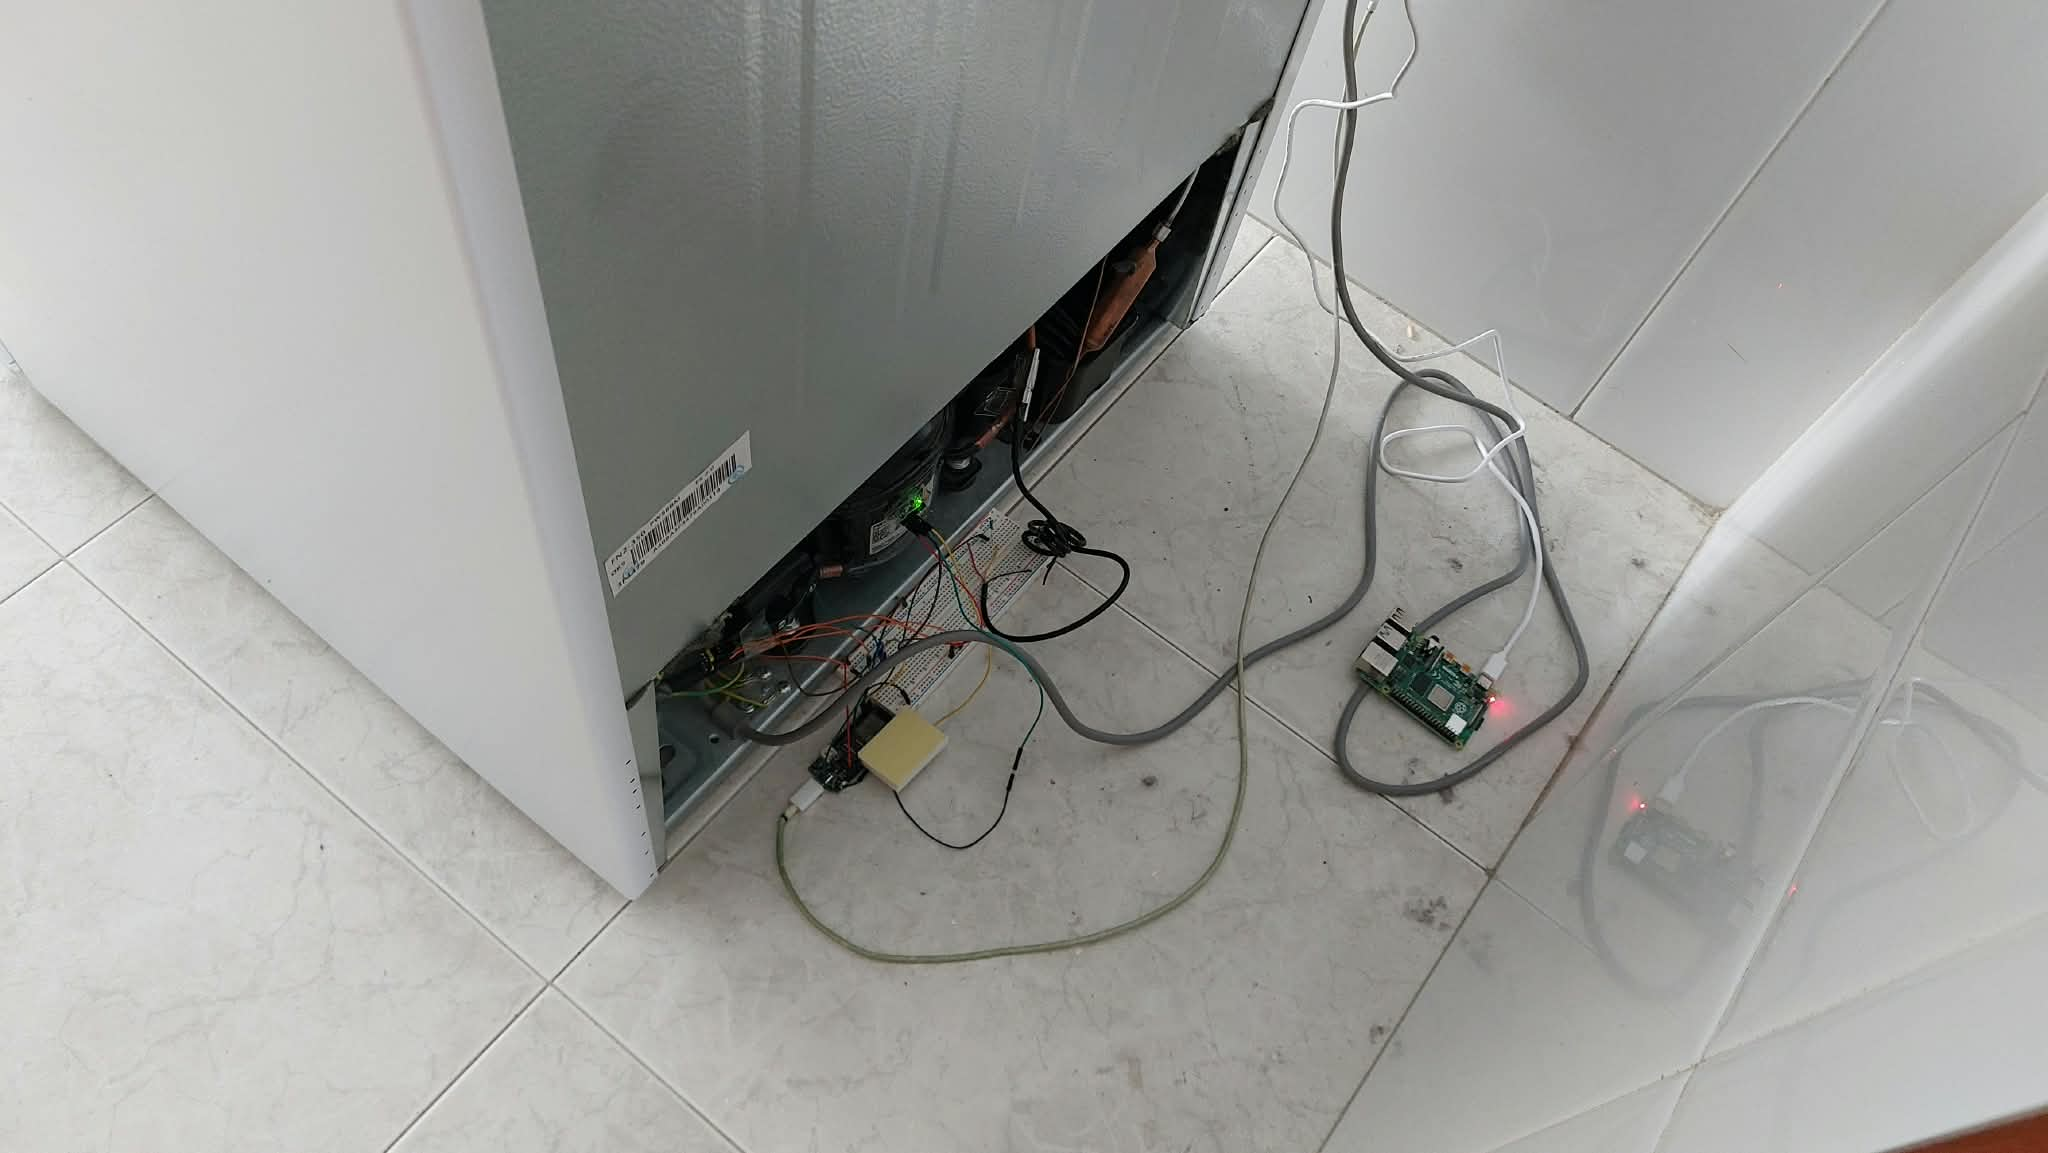
\includegraphics[width=0.92\textwidth]{figuras/banco-conjunto-hub.jpg}
\caption{Conjunto del banco de pruebas: activo de refrigeración, nodo de captura en su base
y concentrador Raspberry~Pi.}
\label{fig:banco-conjunto}
\end{figure}

La figura~\ref{fig:banco-fijacion} recoge el detalle de la fijación del acelerómetro sobre
el compresor del activo de referencia. El sensor se adhiere al lateral de la cúpula del
compresor hermético, y el cableado del bus discurre hasta la placa de prototipado situada en
la base del alojamiento.

\begin{figure}[ht!]
\centering
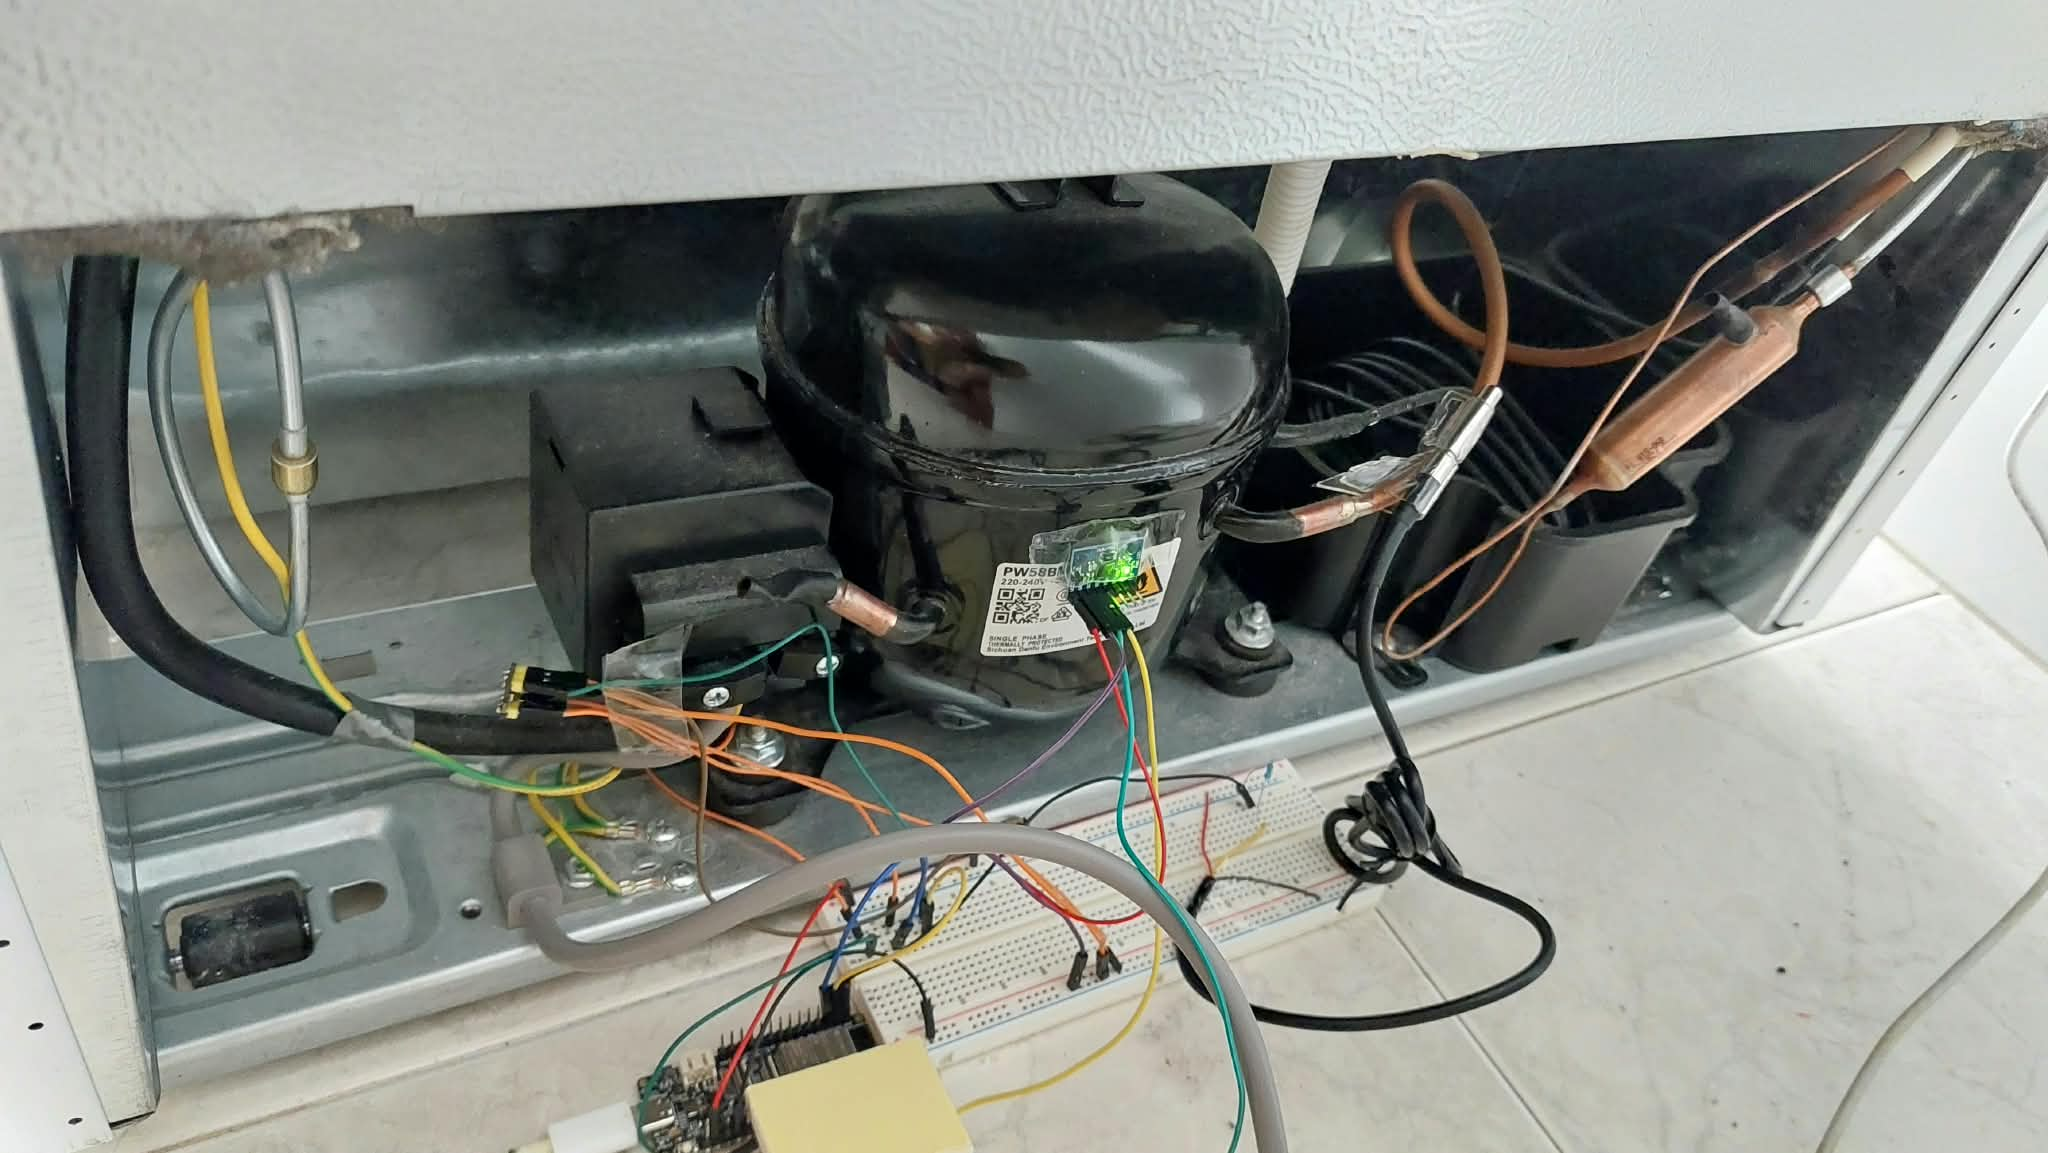
\includegraphics[width=0.92\textwidth]{figuras/banco-fijacion-sensor.jpg}
\caption{Detalle de la fijación del acelerómetro sobre la cúpula del compresor y del
cableado del bus I\textsuperscript{2}C hasta la placa de prototipado.}
\label{fig:banco-fijacion}
\end{figure}

\section{Selección del punto de medida}

La posición del acelerómetro resultó ser la decisión con mayor efecto sobre la calidad de la
medida, por encima del tipo de fijación. La figura~\ref{fig:puntos-medida} señala los tres
puntos evaluados sobre el compresor.

\begin{figure}[ht!]
\centering
\begin{tikzpicture}
  \node[inner sep=0] (foto)
    {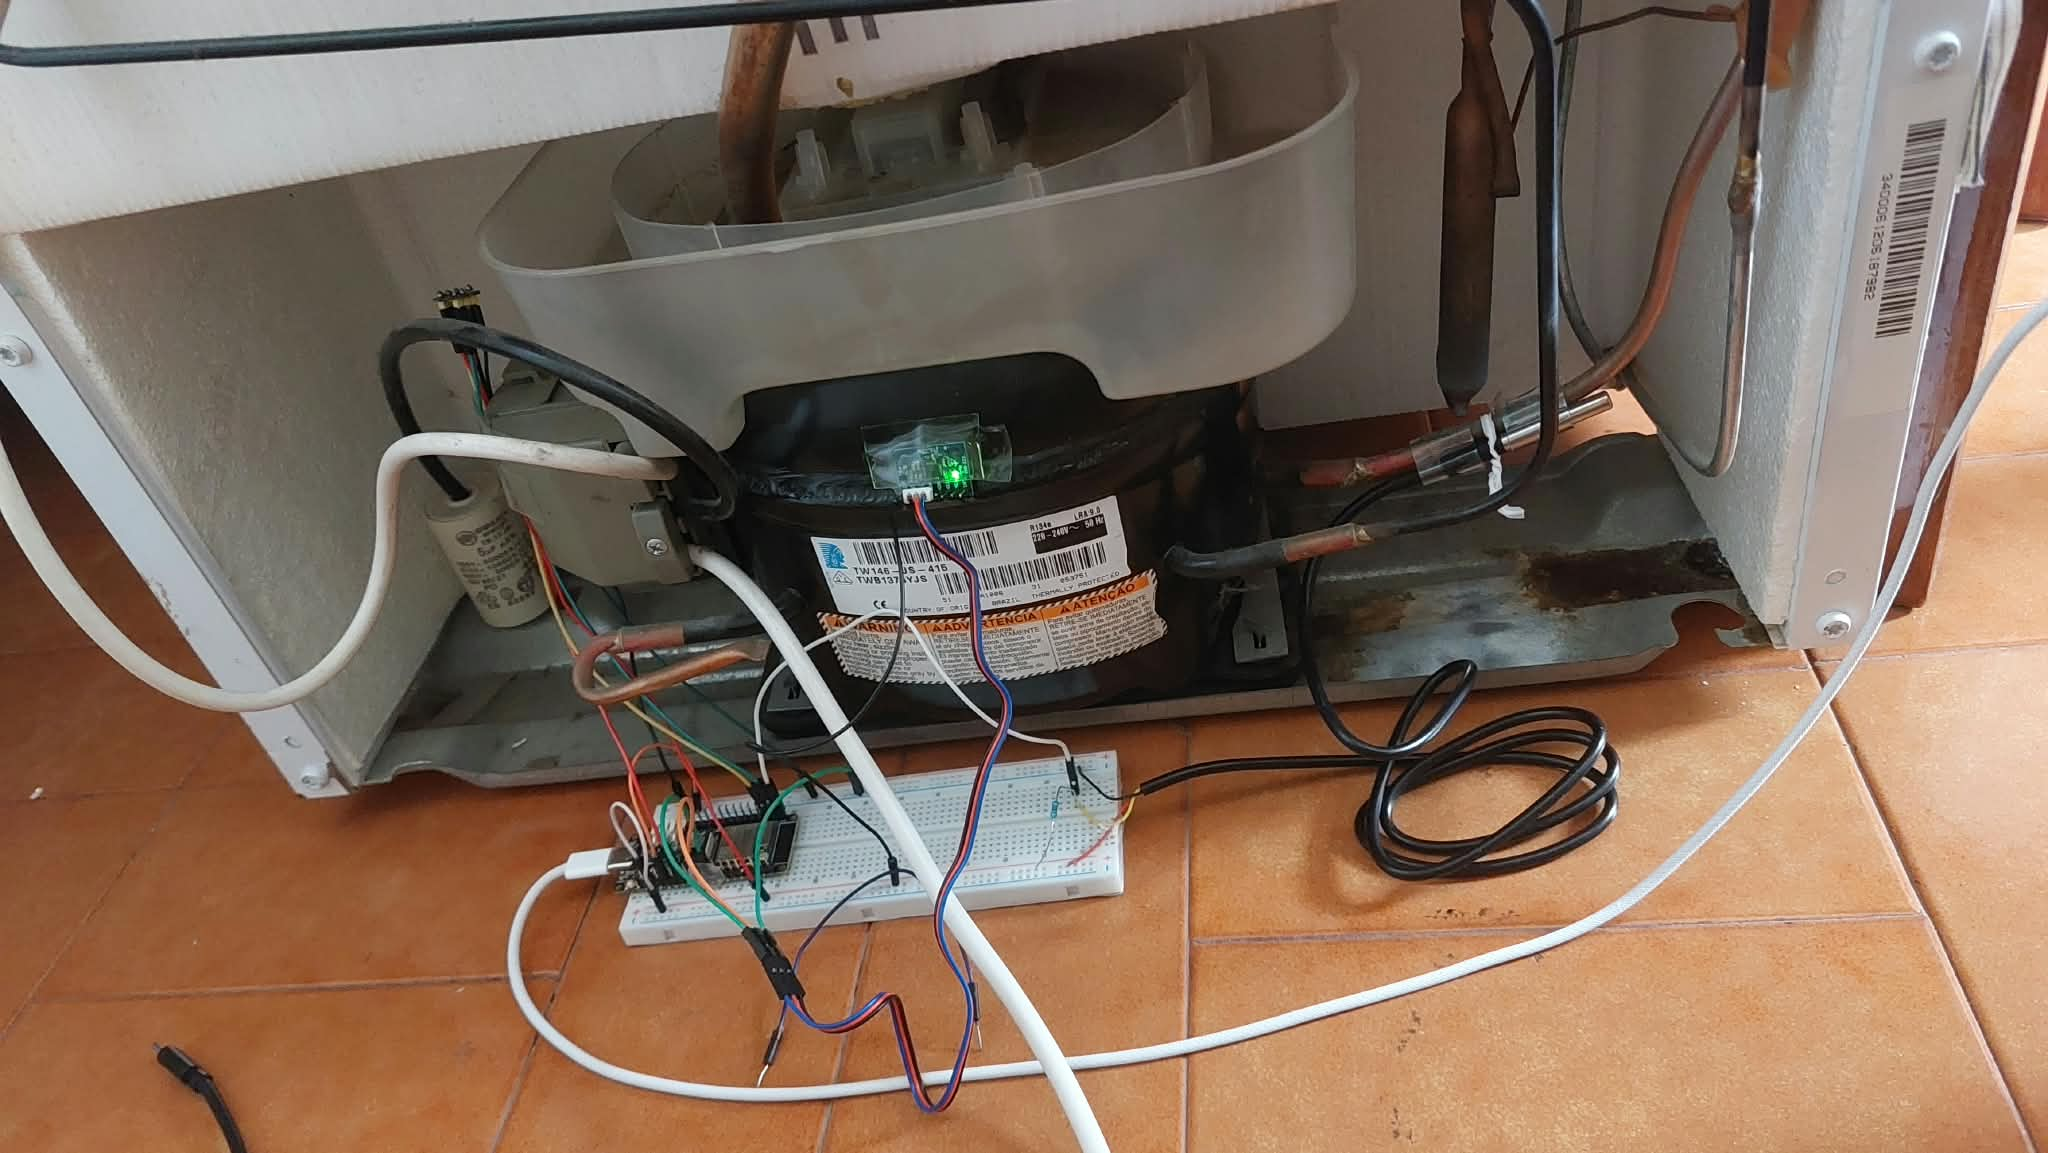
\includegraphics[width=0.94\textwidth]{figuras/banco-compresor-antiguo.jpg}};
  \begin{scope}[x={(foto.south east)}, y={(foto.north west)},
                marca/.style={circle, draw, line width=1.1pt, minimum size=15pt},
                etiq/.style={circle, fill, text=white, font=\bfseries\small,
                             inner sep=1.6pt, minimum size=13pt}]
    % Punto descartado: la cupula del compresor
    \draw[red!75!black, line width=1.1pt, dashed] (0.27,0.80) -- (0.44,0.63);
    \node[marca, red!75!black, minimum size=19pt] at (0.453,0.605) {};
    \node[red!75!black, font=\bfseries] at (0.453,0.605) {$\times$};
    \node[etiq, fill=red!75!black] at (0.255,0.815) {$\times$};

    % Punto 1: pata o anclaje al chasis
    \draw[orange!85!black, line width=1.1pt] (0.78,0.24) -- (0.63,0.40);
    \node[marca, orange!85!black] at (0.607,0.417) {};
    \node[etiq, fill=orange!85!black] at (0.795,0.225) {1};

    % Punto 2: tubo de descarga, el adoptado
    \draw[teal!80!black, line width=1.4pt] (0.17,0.24) -- (0.31,0.40);
    \node[marca, teal!80!black, line width=1.6pt, minimum size=17pt] at (0.326,0.421) {};
    \node[etiq, fill=teal!80!black] at (0.155,0.225) {2};
  \end{scope}
\end{tikzpicture}
\caption{Puntos de medida evaluados sobre el compresor. La cruz marca la cúpula, descartada;
el punto 1 el anclaje al chasis; el punto 2 el tubo de descarga, finalmente adoptado.}
\label{fig:puntos-medida}
\end{figure}

El cuadro~\ref{table:puntos-medida} recoge el resultado de la comparación.

\begin{table}[ht!]
\caption{Comparación de los puntos de medida evaluados.}
\label{table:puntos-medida}
\centering
\begin{tabular}{|p{3.4cm}|p{2.2cm}|p{2.4cm}|p{4.4cm}|}
\hline
\textbf{Punto} & \textbf{Valor eficaz} & \textbf{Fundamental} & \textbf{Resultado} \\
\hline
Cúpula del compresor & \mbox{0,047 m/s$^2$} & 4 de 52 ráfagas & Descartado \\
\hline
Tubo de descarga & \mbox{0,35--0,69 m/s$^2$} & 6 de 7 ráfagas & \textbf{Adoptado} \\
\hline
\end{tabular}
\end{table}

El motivo del descarte de la cúpula es de diseño del propio activo: un compresor hermético
lleva el conjunto motor-bomba suspendido sobre muelles \textit{dentro} de la carcasa, solución
que reduce el ruido transmitido y que, en consecuencia, aísla la superficie exterior de la
vibración que interesa medir. Midiendo en la cúpula se mide por el lado amortiguado de esa
suspensión.

El tubo de descarga, en cambio, está unido rígidamente al cuerpo de la bomba y transporta la
pulsación sin atravesar la suspensión interna. El cambio elevó el valor eficaz entre nueve y
veinte veces según el eje, y la frecuencia fundamental pasó de identificarse en el 8 \% de
las ráfagas a hacerlo en la práctica totalidad.

Procede precisar cómo se reparte esa mejora entre las características, porque el dato en
bruto induce a error. En torno al 95 \% del incremento reside en la componente tonal de alta
frecuencia analizada en el capítulo~\ref{cap:diseno}: el valor eficaz en la banda que
describen los estadísticos temporales es de \mbox{0,062 m/s$^2$} frente a los
\mbox{0,35 m/s$^2$} sin filtrar, de modo que la ganancia sobre esos estadísticos es de un
factor próximo a 1,6 y no de quince. La parte restante no es sin embargo señal desechable:
corresponde a la banda donde el capítulo~\ref{cap:resultados} identifica la firma del fallo.

La figura~\ref{fig:banco-antiguo} corresponde al montaje empleado durante la fase de
depuración del firmware, sobre un segundo activo de mayor antigüedad. Se incluye porque las
incidencias de integridad del bus descritas en el capítulo~\ref{cap:diseno} se
caracterizaron sobre este montaje.

\begin{figure}[ht!]
\centering
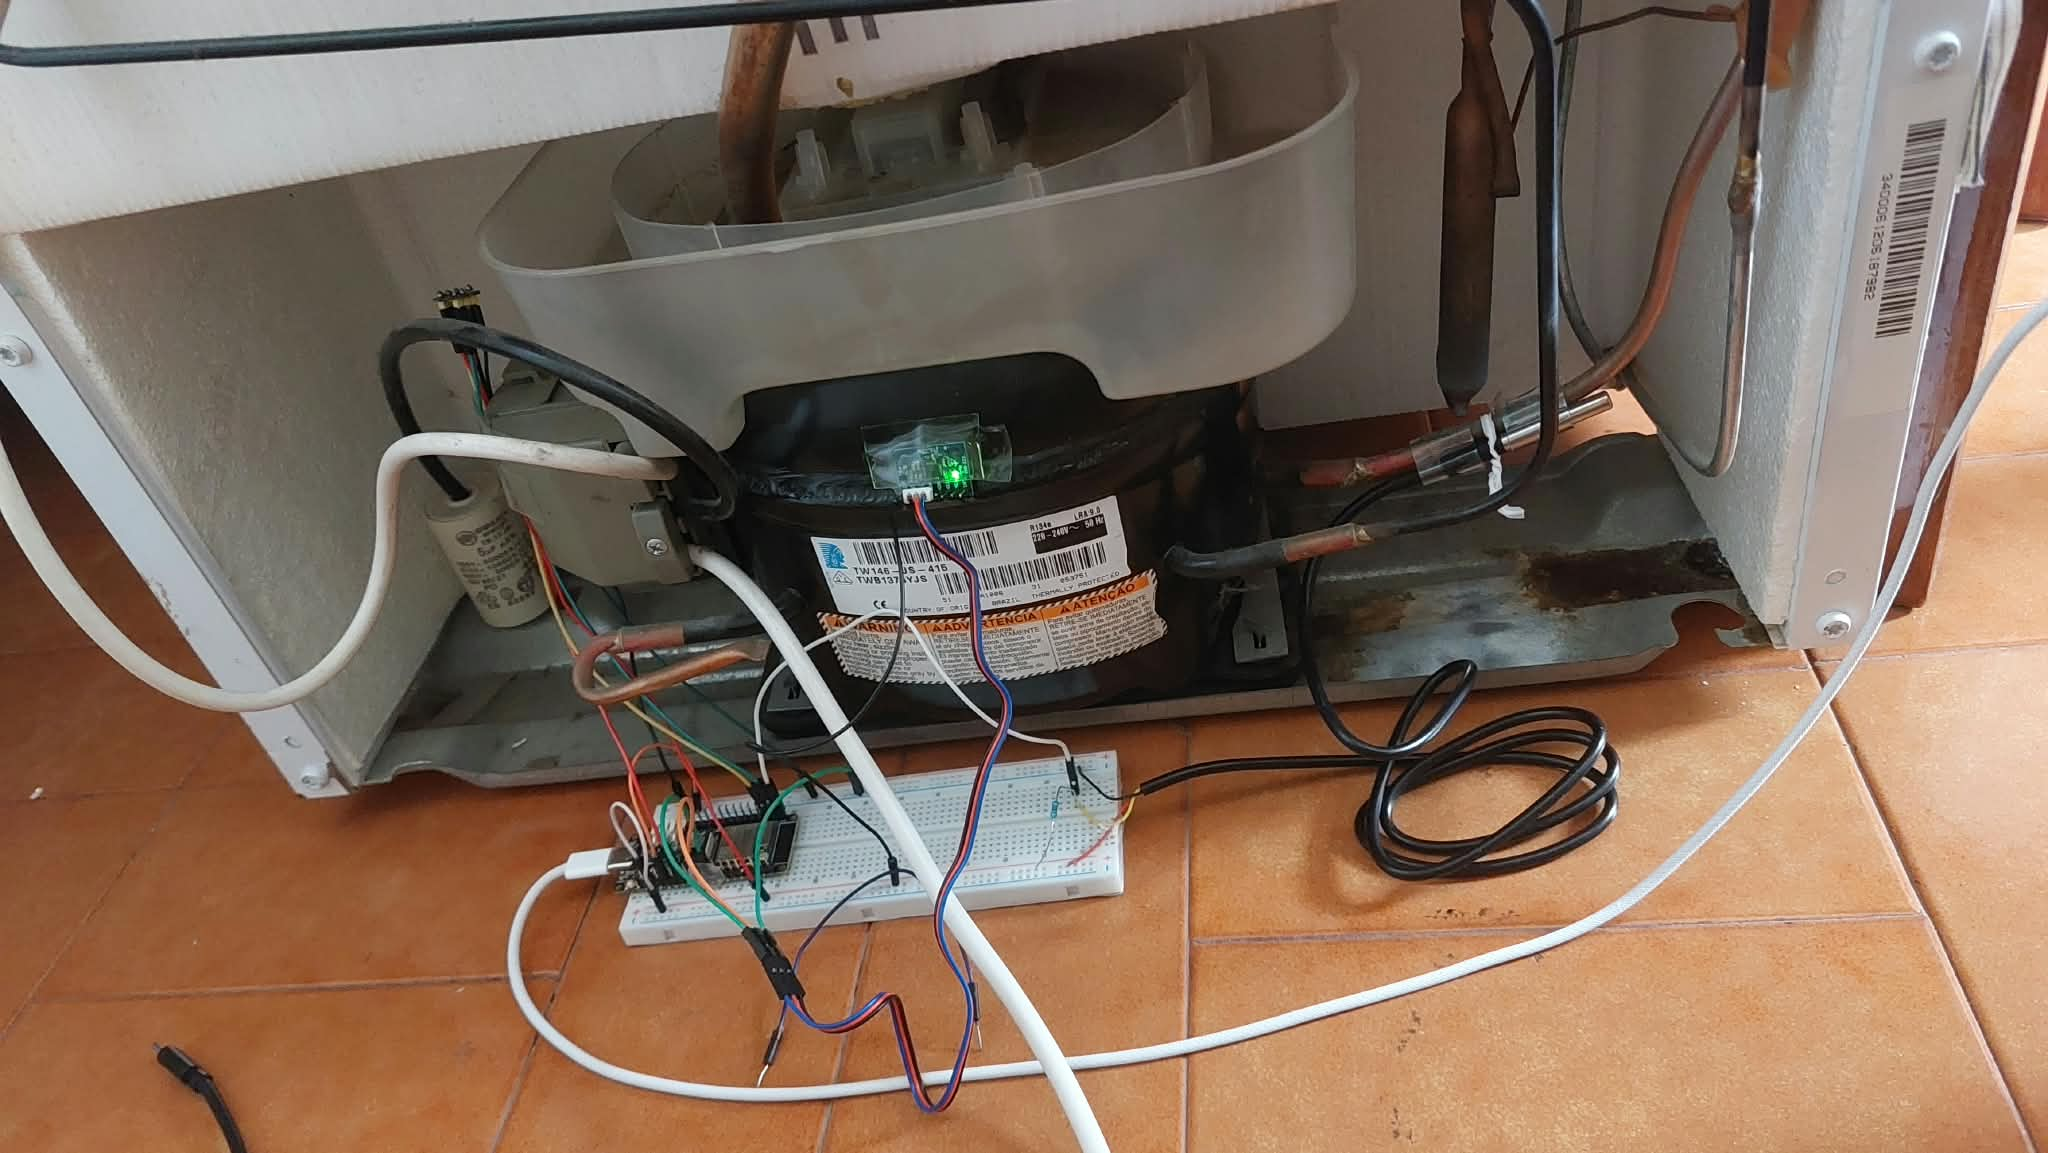
\includegraphics[width=0.92\textwidth]{figuras/banco-compresor-antiguo.jpg}
\caption{Montaje empleado en la fase de depuración, sobre un compresor de mayor antigüedad.}
\label{fig:banco-antiguo}
\end{figure}

\section{Limitaciones del montaje y su efecto sobre la medida}

Procede documentar de forma explícita las limitaciones del montaje, dado que condicionan la
calidad alcanzable del conjunto de datos y la interpretación de los resultados.

El acoplamiento del acelerómetro es adhesivo sobre una superficie curva, no una fijación
rígida atornillada. Una unión de este tipo se comporta como un acoplamiento elástico y
atenúa de forma selectiva el contenido de frecuencia más alta, que es precisamente el
informativo para el diagnóstico. La consecuencia esperable es una subestimación de la
amplitud de vibración y una reducción de la capacidad de discriminación del modelo.

El cableado del bus I\textsuperscript{2}C se realiza con conductores de prototipado sobre
placa de inserción, con una longitud del orden de \mbox{30 cm}, y discurre en paralelo al
cableado de alimentación del compresor, según se aprecia en la
figura~\ref{fig:banco-fijacion}. Este montaje presenta dos consecuencias medidas. La primera
es una tasa de fallo de lectura elevada, del orden de 37 reintentos por minuto con el activo
en marcha, atribuible a la pérdida intermitente de contacto en los conectores por efecto de
la vibración. La segunda es la posibilidad de acoplamiento de la frecuencia de red por
proximidad de conductores, circunstancia relevante porque el régimen de giro del compresor y
la frecuencia de red distan menos de dos veces la resolución espectral del análisis.

Estas limitaciones responden al alcance del trabajo, orientado a demostrar la viabilidad del
enfoque sobre una plataforma de prototipado, y no a producir un dispositivo de instalación
permanente. La decisión adoptada consiste en \textit{asumir} la tasa de fallo del cableado y
compensarla en el firmware mediante la validación de la transacción y el reintento acotado
descritos en el capítulo~\ref{cap:diseno}, en lugar de intervenir sobre el montaje físico. El
coste de esa decisión es una fracción de medidas descartadas mayor de la que tendría un
montaje soldado, cuantificada mediante los contadores de salud que el propio nodo publica.
Una implantación industrial exigiría conexiones soldadas con alivio de tensión y fijación
atornillada del sensor al chasis.

\section{Nota sobre los pines de configuración de arranque}

El pin GPIO~12 empleado para la señal de selección de canal del micrófono actúa como pin de
configuración de arranque en numerosas placas basadas en ESP32. Si la placa no arranca con
el micrófono conectado, procede reasignar esa señal a otra línea disponible.

% I. Anexo técnico: software (Guía apdo. 3.I)
% Fuentes de verdad: docs/DATA_SCHEMA.md, device/device.ino, server/mqtt_logger.py
\chapter{Anexo técnico: software y formato de datos}
\label{anexo:software}

\section{Formato de la trama de telemetría}

El nodo publica en el tema \texttt{fridge/sensors} un objeto JSON con nueve variables por
ciclo de medida. El listado~\ref{listado:trama} muestra un ejemplo de trama.

\begin{lstlisting}[caption=Ejemplo de trama de telemetria publicada por el nodo.,label=listado:trama]
{"tempExt":4.31,"accX":0.12,"accY":-0.05,"accZ":9.79,
 "gyroX":0.01,"gyroY":0.00,"gyroZ":-0.02,"motorTemp":38.6,"noise":142}
\end{lstlisting}

El cuadro de las nueve variables de este canal, con su unidad e intervalo, figura en el
capítulo~\ref{cap:diseno}. El canal de ráfaga, publicado en el tema
\texttt{fridge/vibration}, transporta en cambio características ya calculadas y no medidas
instantáneas. El cuadro~\ref{table:rafaga} recoge su contenido completo.

\begin{table}[ht!]
\caption{Campos del canal de ráfaga. El sufijo \texttt{\_x}, \texttt{\_y} o \texttt{\_z}
identifica el eje.}
\label{table:rafaga}
\centering
\begin{tabular}{|p{2.6cm}|p{1.5cm}|p{8.3cm}|}
\hline
\textbf{Campo} & \textbf{Unidad} & \textbf{Contenido} \\
\hline
\texttt{vib\_fs} & Hz & Frecuencia de muestreo de la ráfaga (1000) \\
\hline
\texttt{vib\_n} & --- & Muestras por ráfaga (1024) \\
\hline
\texttt{ms\_capture} & ms & Duración real de la captura. Es el control de calidad de la
ráfaga: una desviación respecto de \mbox{1024 ms} comprime el eje de frecuencias \\
\hline
\texttt{ms\_total} & ms & Captura más cálculo de características \\
\hline
\texttt{failed\_bursts} & --- & Ráfagas descartadas acumuladas \\
\hline
\texttt{bad\_frames} & --- & Tramas del canal lento descartadas acumuladas \\
\hline
\texttt{retries} & --- & Reintentos de lectura en la ráfaga en curso \\
\hline
\texttt{total\_retries} & --- & Reintentos acumulados desde el arranque \\
\hline
\texttt{rms\_*} & m/s$^2$ & Valor eficaz de la componente alterna \\
\hline
\texttt{peak\_*} & m/s$^2$ & Máximo absoluto tras eliminar la continua \\
\hline
\texttt{kurt\_*} & --- & Kurtosis. 3 para ruido gaussiano, 1,5 para senoide pura \\
\hline
\texttt{fdom\_*} & Hz & Frecuencia dominante, refinada por interpolación parabólica \\
\hline
\texttt{adom\_*} & m/s$^2$ & Amplitud estimada en la frecuencia dominante \\
\hline
\texttt{aud\_fs} & Hz & Frecuencia de muestreo del audio (16000) \\
\hline
\texttt{aud\_n} & --- & Muestras de audio analizadas \\
\hline
\texttt{aud\_rms} & --- & Valor eficaz de la señal acústica, en unidades relativas \\
\hline
\texttt{aud\_b0} a \texttt{aud\_b3} & --- & Fracción de energía espectral en las bandas
0--250, 250--1000, 1000--4000 y 4000--8000 \mbox{Hz}. Las cuatro suman la unidad \\
\hline
\end{tabular}
\end{table}

Las cuatro bandas acústicas expresan fracciones y no niveles absolutos: describen cómo se
reparte la energía del sonido, no cuánta hay. El nivel absoluto reside en \texttt{aud\_rms}.

\section{Valores centinela y tratamiento de datos ausentes}

El sistema distingue explícitamente entre una medida válida y la ausencia de medida. Un
valor de \mbox{$-127$ \textdegree C} en la temperatura externa indica sonda desconectada, y
un bloque de siete variables del acelerómetro con valor exactamente nulo indica que el bus
I\textsuperscript{2}C no pudo recuperarse en ese ciclo. Ambos casos deben filtrarse antes
de calcular cualquier estadístico, ya que su inclusión distorsiona los promedios del
conjunto de datos.

\section{Dependencias del entorno de desarrollo}

El cuadro~\ref{table:dependencias} recoge las versiones empleadas, tomadas del registro de
compilación del firmware y del fichero de dependencias del concentrador. Se documentan de
forma explícita porque el comportamiento de una de ellas resultó determinante para el diseño
de la adquisición, según se describe en el capítulo~\ref{cap:diseno}.

\begin{table}[ht!]
\caption{Versiones del entorno de desarrollo y de las dependencias.}
\label{table:dependencias}
\centering
\begin{tabular}{|p{5.4cm}|p{2.4cm}|p{4.4cm}|}
\hline
\textbf{Componente} & \textbf{Versión} & \textbf{Función} \\
\hline
Núcleo Arduino para ESP32 & 3.3.1 & Entorno de ejecución del nodo \\
\hline
Wire & 3.3.0 & Bus I\textsuperscript{2}C \\
\hline
Adafruit MPU6050 & 2.2.9 & Configuración del acelerómetro \\
\hline
Adafruit BusIO & 1.17.4 & Abstracción de bus \\
\hline
Adafruit Unified Sensor & 1.1.15 & Interfaz común de sensores \\
\hline
OneWire & 2.3.8 & Bus 1-Wire \\
\hline
DallasTemperature & 4.0.6 & Sonda DS18B20 \\
\hline
WiFi / Networking & 3.3.0 & Conectividad del nodo \\
\hline
PubSubClient & 2.8 & Cliente MQTT del nodo \\
\hline
Python & 3.11 o superior & Entorno del concentrador \\
\hline
paho-mqtt & 2.1.0 & Cliente MQTT del registrador \\
\hline
python-dotenv & 1.0.1 & Configuración por variables de entorno \\
\hline
Mosquitto & 2.0 o superior & Intermediario de mensajería \\
\hline
\end{tabular}
\end{table}

La biblioteca Adafruit MPU6050 se emplea únicamente para la configuración inicial del
sensor, y no para la lectura de medidas. El motivo es que su función de obtención de datos
devuelve un indicador de éxito incondicional y opera sobre un almacén no inicializado, de
modo que ante un fallo del bus entrega como medida el contenido residual de la pila. La
lectura se realiza por ello mediante acceso directo a los registros del dispositivo, con la
validación descrita en el capítulo~\ref{cap:diseno}. Se documenta esta circunstancia porque
condiciona la reproducibilidad: una implementación que confiara en esa biblioteca para la
adquisición reproduciría el mismo defecto.

\section{Aprovisionamiento del concentrador}

El capítulo~\ref{cap:metodologia} expone los criterios que rigen el despliegue; esta sección
recoge el procedimiento reproducible. El aprovisionamiento está automatizado en un
\textit{script} que admite ejecutar las operaciones de una vez o por fases separadas, según
el listado~\ref{lst:aprovisionamiento}.

\begin{lstlisting}[caption={Aprovisionamiento completo del concentrador.}, label={lst:aprovisionamiento}]
# Desde el equipo de desarrollo: copiar el proyecto al concentrador.
# Se excluyen el entorno virtual, la configuracion local y los datos
# capturados, para no sobrescribir lo que ya reside en el concentrador.
rsync -av --exclude .venv --exclude 'server/.env' --exclude 'server/data' \
      <ruta-local>/ <usuario>@<direccion>:/home/<usuario>/TFM/

# En el concentrador: aprovisionamiento completo
cd ~/TFM
sudo AP_PASS='<clave-de-la-red>' ./server/provision-pi.sh todo
\end{lstlisting}

El cuadro~\ref{table:fases-aprovisionamiento} detalla las operaciones y su orden, que no es
arbitrario.

\begin{table}[ht!]
\caption{Fases del aprovisionamiento del concentrador.}
\label{table:fases-aprovisionamiento}
\centering
\begin{tabular}{|p{2.1cm}|p{10.4cm}|}
\hline
\textbf{Fase} & \textbf{Operación} \\
\hline
\texttt{paquetes} & Instalación del intermediario de mensajería y del entorno de ejecución
de Python. Requiere acceso a Internet \\
\hline
\texttt{broker} & Configuración del intermediario, con examen previo de la configuración
existente \\
\hline
\texttt{logger} & Entorno virtual, configuración por variables de entorno y declaración del
registrador como servicio del sistema. Incluye una comprobación de extremo a extremo con una
trama sintética \\
\hline
\texttt{ap} & Conversión de la interfaz inalámbrica en punto de acceso. Última operación \\
\hline
\texttt{comprobar} & Verificación de la cadena completa. No requiere privilegios \\
\hline
\texttt{revertir} & Restitución de la interfaz a modo cliente y detención del registrador,
conservando los datos capturados \\
\hline
\end{tabular}
\end{table}

Tres particularidades del procedimiento responden a restricciones del entorno. La primera es
que las comprobaciones previas se completan antes de modificar el sistema, de modo que una
condición no satisfecha aborta la ejecución sin dejar el equipo en un estado intermedio. La
segunda es que la activación del punto de acceso interrumpe la red por la que llega la sesión
de administración remota, por lo que constituye la última operación y se lanza desacoplada de
la sesión mediante el gestor de servicios, con objeto de que se complete aunque la conexión se
pierda; los datos de acceso se escriben en un fichero del concentrador antes de esa
activación, para que puedan consultarse localmente después. La tercera es la existencia de la
fase de reversión, exigible cuando el equipo presta además otros servicios: la
restitución no elimina los ficheros de datos capturados.

La instalación exige acceso a Internet, mientras que el punto de acceso lo suprime en la
interfaz inalámbrica. Ese es el motivo del orden establecido, y no una preferencia
organizativa: invertirlo dejaría el concentrador sin posibilidad de completar la instalación
de dependencias.

\section{Puesta en marcha y verificación del concentrador}

El concentrador no requiere intervención para entrar en servicio. El intermediario de
mensajería, el registrador y el punto de acceso inalámbrico están declarados como servicios
del sistema con arranque automático, de modo que la alimentación eléctrica es la única
condición necesaria. Esta propiedad se estableció como requisito porque una campaña de
adquisición prolongada debe sobrevivir a un corte de suministro sin perder más datos que los
del intervalo sin corriente, y el registrador escribe en modo de adición, con lo que
prosigue el fichero de la jornada en lugar de sustituirlo.

El registrador se declara además con reinicio automático ante terminación anómala. El
criterio subyacente es que los datos en bruto son irrecuperables si se pierden, de modo que
un fallo puntual del proceso no debe interrumpir la campaña.

La verificación de la cadena completa se realiza con el procedimiento recogido en el
listado~\ref{lst:verificacion}, que recorre el camino del dato en el mismo orden en que este
fluye. Esa ordenación es deliberada: el primer eslabón que falla localiza el corte, de forma
que no es necesario examinar los posteriores.

\begin{lstlisting}[caption={Verificacion de la cadena de adquisicion en el concentrador.}, label={lst:verificacion}]
# Verificacion completa: punto de acceso, nodo asociado, intermediario,
# tramas de ambos canales, registrador y crecimiento de los ficheros
./server/provision-pi.sh comprobar

# Seguimiento durante la campana
journalctl -u tfm-logger -f
wc -l server/data/*.csv
\end{lstlisting}

La comprobación del registrador no se limita a constatar la existencia de los ficheros de
datos, sino que contrasta su número de filas en dos instantes separados. La distinción es
pertinente: un fichero presente que no crece constituye un modo de fallo silencioso, y se
observó durante la puesta a punto que puede producirse con el servicio aparentemente activo y
las tramas llegando correctamente al intermediario.

El origen de aquel incidente ilustra un aspecto del comportamiento del sistema operativo que
conviene documentar. Al eliminar los ficheros de datos con el registrador en ejecución, el
descriptor abierto por el proceso continúa referenciando el fichero original, ya desvinculado
del sistema de ficheros, por lo que la escritura prosigue sobre un destino inaccesible
mientras el fichero visible permanece vacío. La reapertura solo se produce al cambiar la
fecha. Se establece por ello como procedimiento que toda manipulación del directorio de datos
se realice con el servicio detenido, según el listado~\ref{lst:limpieza}.

\begin{lstlisting}[caption={Reinicio del directorio de datos antes de una campana.}, label={lst:limpieza}]
D=server/data/descartes-$(date +%Y%m%d-%H%M)
sudo systemctl stop tfm-logger        # detener ANTES de tocar los ficheros
mkdir -p "$D" && mv server/data/*.csv "$D"/
sudo systemctl start tfm-logger       # los recrea con su cabecera
\end{lstlisting}

Los ficheros se archivan en lugar de eliminarse, dado que las capturas de puesta a punto
constituyen la evidencia de las incidencias descritas en el capítulo~\ref{cap:diseno}. Debe
evitarse crear los ficheros de forma manual tras retirarlos: el registrador escribe la
cabecera únicamente cuando el fichero no existe o está vacío, y un fichero preexistente
produciría un conjunto de datos sin nombres de columna.

\section{Procedimiento de despliegue del modelo en el nodo}

El modelo ajustado llega al firmware a través de un fichero de cabecera generado por el entorno
de análisis, según la secuencia siguiente:

\begin{enumerate}
\item El procedimiento de exportación ajusta el modelo sobre el conjunto de referencia y escribe
      \texttt{device/modelo\_referencia.h}, que contiene los parámetros y, en su encabezado, la
      campaña, la duración, el número de ráfagas y episodios, los umbrales del filtro de calidad
      y la fecha de generación.
\item Un segundo procedimiento exporta las ráfagas reales con la puntuación que produce la
      biblioteca de referencia sobre cada una, para contrastar la implementación embarcada.
\item Las rutinas del detector se compilan y verifican en un computador frente a esos valores.
\item Solo entonces se compila el firmware y se programa la placa.
\end{enumerate}

La separación entre los parámetros y las rutinas es deliberada: reentrenar el modelo consiste en
volver a ejecutar la exportación y recompilar, sin modificar código. El fichero generado no se
edita a mano, y su encabezado permite rastrear cualquier firmware programado en una placa hasta
los datos que lo produjeron.

\section{Especificidad del modelo respecto del activo}

Procede consignar una restricción de despliegue que el propio procedimiento de verificación puso
de manifiesto. El modelo exportado incorpora las medianas del activo sobre el que se ajustó, su
umbral de discriminación entre marcha y parada y su referencia de estado nominal. Programarlo en
un nodo instalado sobre otro activo produce la declaración de medida no evaluable en la
totalidad de las ráfagas: se comprobó que el activo con fallo presenta un valor eficaz en marcha
de \mbox{0,16 m/s$^2$} frente al umbral de \mbox{0,199 m/s$^2$} derivado del activo de
referencia, de modo que sus ráfagas se clasifican como capturadas con el compresor detenido.

\textbf{El modelo es específico del activo}, y cada nodo requiere su propia campaña de
referencia. De ello se sigue asimismo que el nodo necesita una fase de referencia antes de poder
emitir su primer veredicto, dado que las características normalizadas por el propio activo
exigen conocer su mediana.

\section{Rutina de recuperación del bus}

El listado~\ref{lst:recuperacion} recoge la rutina completa. Se invoca cuando una lectura ha
fallado de forma efectiva, y no de forma preventiva en cada ciclo.

\begin{lstlisting}[language=C++, caption={Rutina de recuperacion del bus I2C.}, label={lst:recuperacion}]
bool recoverI2C() {
  Wire.end();
  delay(100);
  Wire.begin(I2C_SDA, I2C_SCL);
  Wire.setClock(I2C_FREQ_HZ);

  if (mpu.begin()) {
    mpu.setAccelerometerRange(MPU6050_RANGE_4_G);
    mpu.setFilterBandwidth(MPU6050_BAND_260_HZ);
    mpu.setSampleRateDivisor(0);
    delay(50);            // los registros valen 0 hasta la 1a conversion
    updateGyroScale();    // begin() reprograma el rango del giroscopo
    return true;
  }
  return false;
}
\end{lstlisting}

Tres aspectos del listado responden a incidencias detectadas en la placa. Los pines del bus
se indican de forma explícita en la reapertura, en lugar de heredarse de la configuración de
la variante de la placa, para que la recuperación no reasigne el bus a pines distintos de los
cableados. La espera posterior a la reinicialización es necesaria porque la puesta en marcha
del sensor conlleva un reinicio del dispositivo, tras el cual sus registros de medida
permanecen a cero hasta que concluye la primera conversión; leerlos antes introduciría
muestras nulas indistinguibles de una medida. Por último, la escala del giroscopio se vuelve
a consultar al dispositivo, dado que la reinicialización reprograma su fondo de escala y
suponerlo en lugar de leerlo alteraría de forma silenciosa las unidades de tres variables del
conjunto de datos.


% **************************************************
% * Bibliografía — H. Estilo IEEE (referencias.bib)
% **************************************************
\bibliographystyle{IEEEtran}
\bibliography{referencias}

\end{document}
